\chapter{Channel atlas}\label{chap:9}
A dark-matter particle of \SI{1}{MeV} brings at most \SI{3.5}{eV} of kinetic energy into a silicon crystal (\cref{sec:1.3}). That is enough to lift an electron across the gap of \SI{1.17}{eV}, or to create an optical phonon of \SI{64.1}{meV}, or, if the particle couples to nucleons, to make a nucleus recoil, which now and then leaves its electrons excited (the Migdal effect). Which of these happens depends on what the particle couples to and on its mass. GaAs has polar phonons that a dark photon sees, an antiferromagnet has spin waves that only a spin coupling creates, and aluminum has broken Cooper pairs at \SI{0.36}{meV}. \Cref{chap:8} gave the rate for all of them: every coupling reduces to a few target operators, the rate contracts their response with a tensor of the dark-matter model, and the final states split into sectors so that none is counted twice. The chapters that follow apply it to two dozen kinds of excitation and six classes of coupling. At that size the hazard is counting a process twice or not at all. The literature computes many channels with formulas of its own, and a process can enter two of them: phonon-assisted absorption above the direct gap contains a cascade that direct absorption counts again (\cref{sec:6.5}). A process can also enter none, as the spin flip of a core electron by a spin coupling enters none of the rates of the following chapters.

A dark photon reaches the electrons and the polar phonons of GaAs through one charge response, and adding its electron-recoil rate to its phonon rate counts the same final states twice unless the sectors of \cref{sec:8.6} keep them apart. A detector that counts pairs in silicon reaches masses from 0.333 to \SI{0.405}{MeV} through pairs created together with a phonon, which a zero-phonon rate does not contain. And a published formula that is accurate for one material and one range of momentum transfer is used outside both, unless something records where it fails. Before any rate is computed, we therefore fix for each pairing of an excitation with a coupling the section that computes it, the lightest dark-matter mass it reaches and where its final states lie on the plane of momentum transfer and energy deposit.

\section{The excitation--interaction matrix}\label{sec:9.1}

\Cref{tab:9-atlas} has 24 rows, one for each kind of excitation that this book treats, and six columns, one for each class of dark-matter coupling. Of its 144 cells, 57 hold a channel, and each of those names the one section that computes its rate. Eight more are allowed at leading order but computed in no section. The remaining 79 are empty at leading order, for reasons of operator content, kinematics or order in the coupling that we work out below. A channel is a pair of row and column, so the table is also a check that no channel is computed twice: where two sections seem to treat the same process, they treat different cells, or different parts of one response.

\subsection{Excitation and interaction axes}\label{sec:9.1-axes}

The columns come from the reduction of \cref{sec:8.1}. Every slow interaction, written in the operator basis $\mathcal{O}_1,\dots,\mathcal{O}_{15}$, reduces to a few target operators per species $s$: the number density $n_s$, the spin density $\vect{s}_s$, the paramagnetic current $\vect{j}_s$, the spin current $\mathcal{J}^{\alpha\beta}_s$ and the kinetic-energy density $\mathcal{T}_s$ (\cref{eq:8.1-rows,tab:8-operators}). Three distinctions separate the columns. The first is scattering against absorption. A scattered particle deposits $\omega$ over a region of the $(\vect{q},\omega)$ plane bounded by the kinematics of \cref{sec:1.3}, while an absorbed boson deposits its mass at the single point $\vect{q} = \vect{p}_\phi = m_\phi\vect{v}$, $\omega = m_\phi$ (\cref{sec:8.1-kinematics,sec:8.2-absorption}). The second is the species: the electron rows and the nuclear rows reach different final states, as \cref{sec:8.6} showed. The third is the operator: a density cannot flip a spin, and a spin density carries no charge.

\emph{Electron density} holds every scattering coupling whose leading target operator is $n_e$, for a heavy or a light mediator: $\mathcal{O}_1$ with the coefficient $c_1^{(e)} = \tilde V$, and the density parts of $\mathcal{O}_5$, $\mathcal{O}_8$ and $\mathcal{O}_{11}$. \emph{Nuclei} holds the couplings to $n_\kappa$, with the coherent weight $Zc_1^{(p)} + (A - Z)c_1^{(n)}$ of \cref{eq:8.1-nuclear}. \emph{Spin and current} holds the couplings to $\vect{s}_s$, $\vect{j}_s$ and $\mathcal{J}^{\alpha\beta}_s$, of electrons or of nuclei: $\mathcal{O}_4$ and the other operators of \cref{tab:8-operators} marked as flipping spins, and the current parts of $\mathcal{O}_2$, $\mathcal{O}_5$ and $\mathcal{O}_8$. In the lattice rows its cells are those of the nuclear spin. \emph{Vector absorption} is the absorption of a dark photon, whose row $-\vect{j}_e + \sum_\kappa Z_\kappa\vect{j}_\kappa$ is the current of all charges, or of another vector boson. \emph{Axion-like and scalar absorption} uses $\vect{s}_e$ and the trace $\mathcal{J}^{\alpha\alpha}_e$ for the axion-like particle (\cref{eq:8.1-alp}) and $n_e - \mathcal{T}_e/m_e$ for the scalar (\cref{eq:8.1-scalar}), or their nucleon analogues.

The last column keeps the target rows and changes the kinematics. It collects inelastic dark matter with a mass splitting $\Delta_\chi$ (\cref{eq:8.1-omega-inel}) and its exothermic version, which deposits more than its kinetic energy (\cref{sec:8.2-exothermic}). It also collects dark matter boosted to relativistic speed, and fermionic absorption, in which the dark matter turns into a light fermion and deposits energy along the line $\omega = \mchi - q$ (\cref{eq:8.1-omega-ferm}). A coupling to the electron density thus belongs to the first column when the dark matter scatters elastically and to the last when it scatters inelastically. The last column, however, holds a cell only where the change of kinematics changes the physics (\cref{sec:9.1-empty}).

The rows follow the solid-state sectors of \crefrange{chap:3}{chap:7}, in the order in which the channel chapters take them up. Electronic excitations at clamped nuclei come first, then lattice excitations, then the mixed processes in which a phonon and an electronic excitation are created together, and last the magnetic, superconducting and other targets. \Cref{tab:9-atlas} cites their defining sections. One row is new. \emph{Phonon-assisted electron recoil} is the creation of an electron--hole pair together with a phonon, which supplies crystal momentum that the dark matter cannot. It is the scattering counterpart of the phonon-assisted absorption of light in \cref{sec:6.5}, and \cref{sec:13.2}, which derives its second-order amplitude, makes it precise. In silicon it is the only way that dark matter scattering on electrons can create a pair at masses just below the zero-phonon threshold, because the gap is indirect (\cref{sec:3.3}). Rows that none of those chapters introduces carry a one-line description.

\begin{table}[tbp]
  \centering
  \footnotesize
  \setlength{\tabcolsep}{2.5pt}
  \renewcommand{\arraystretch}{1.05}
  \caption{The channel atlas. Rows: excitations of a solid, with their defining section or a short description. Sector: the final-state sector of \cref{eq:8.6-partition} (\cref{sec:8.6}). ad: electron-following; 0: zero-phonon electronic; $+$: phonon-dressed electronic; ad$^{\mathrm{s}}$: electron-following on the spin manifold of a magnet; qp: the quasiparticle-number sectors of a gapless target; $(2,0)$: pair breaking, and $(2,m)$ pair breaking with $m$ phonons. Columns: classes of coupling, with the target operators of \cref{sec:8.1}; ALP: axion-like particle; abs.: absorption. Entry: the one section that computes the rate; $\circ$: allowed at leading order, computed in no section; ---: no channel at leading order (\cref{sec:9.1-empty}). The density cell of single phonons is the coupling to charge through the Born charges; for a coupling to electrons alone, the acoustic peak of the electrons that follow the nuclei is computed in \cref{sec:10.2}. The absorption cells of excitons rest on measured optical data.}
  \label{tab:9-atlas}
  \begin{tabular}{@{}>{\raggedright\arraybackslash}p{0.31\linewidth}>{\centering\arraybackslash}p{0.068\linewidth}*{6}{>{\centering\arraybackslash}p{0.085\linewidth}}@{}}
    \toprule
    Excitation & Sector & Electron density & Nuclei & Spin, current & Vector abs. & ALP, scalar abs. & Inelastic, other \\
    & & $n_e$ & $n_\kappa$ & $\vect{s}$, $\vect{j}$, $\mathcal{J}$ & $\vect{j}_e$, $\vect{j}_\kappa$ & $\vect{s}_e$, $\mathcal{J}^{\alpha\alpha}_e$, $\mathcal{T}_e$ & rows of $\vect{q}$, $\Delta_\chi$ \\
    \midrule
    Electron--hole pairs, band to band (\ref{sec:3.2}, \ref{sec:4.2}) & 0 & \ref{sec:10.1} & --- & \ref{sec:10.4} & \ref{sec:10.7} & \ref{sec:10.7} & \ref{sec:10.9} \\
    Electron-gas continua and plasmons (\ref{sec:4.5}) & 0; qp & \ref{sec:10.3} & --- & --- & \ref{sec:10.7} & --- & \ref{sec:17.3} \\
    Excitons (\ref{sec:4.9}) & 0 & \ref{sec:10.5} & --- & \ref{sec:10.5} & \ref{sec:10.7} & \ref{sec:10.7} & --- \\
    Core and semicore electrons (\ref{sec:3.5}) & 0 & \ref{sec:10.6} & --- & $\circ$ & \ref{sec:10.7} & --- & --- \\
    \addlinespace[2pt]
    Single phonons (\ref{sec:5.3}, \ref{sec:5.5}) & ad & \ref{sec:11.2} & \ref{sec:11.1} & \ref{sec:11.6} & \ref{sec:11.8} & \ref{sec:11.8} & \ref{sec:17.3} \\
    Multiphonons (\ref{sec:5.6}) & ad & \ref{sec:11.3} & \ref{sec:11.3} & \ref{sec:11.6} & --- & --- & --- \\
    Free nuclear recoil (\ref{sec:1.3}, \ref{sec:5.6}) & ad & $\circ$ & \ref{sec:11.4} & \ref{sec:11.6} & --- & --- & \ref{sec:11.4} \\
    Quantum crystal: solid helium & ad & --- & \ref{sec:11.5} & --- & --- & --- & --- \\
    \addlinespace[2pt]
    Migdal effect: electrons with a nuclear recoil (\ref{sec:6.1}) & 0, $+$ & --- & \ref{sec:12.3} & $\circ$ & --- & \ref{sec:12.6} & --- \\
    Phonon-assisted electron recoil (\ref{sec:6.5}) & $+$ & \ref{sec:13.3} & --- & $\circ$ & \ref{sec:13.8} & \ref{sec:13.8} & --- \\
    \addlinespace[2pt]
    Magnons (\ref{sec:7.1}) & ad$^{\mathrm{s}}$ & --- & --- & \ref{sec:14.1} & \ref{sec:14.3} & \ref{sec:14.3} & \ref{sec:17.3} \\
    Two-magnon continua, magnon--phonon modes & ad$^{\mathrm{s}}$ & --- & --- & \ref{sec:14.2} & --- & --- & --- \\
    Chiral and nonreciprocal modes: crystals without inversion or time reversal & ad, ad$^{\mathrm{s}}$ & --- & --- & \ref{sec:14.5} & \ref{sec:14.5} & \ref{sec:14.5} & --- \\
    Precessing nuclear spins in a coherent field & ad & --- & --- & --- & --- & \ref{sec:14.6} & --- \\
    \addlinespace[2pt]
    Superconducting quasiparticles (\ref{sec:7.2}) & $(2,0)$, $(2,m)$ & \ref{sec:15.1} & --- & $\circ$ & \ref{sec:15.4} & \ref{sec:15.4} & --- \\
    Dirac and narrow-gap pairs (\ref{sec:7.3}) & qp; 0 & \ref{sec:16.1} & --- & $\circ$ & \ref{sec:16.1} & --- & --- \\
    Plasmons of sheets, wires and layered stacks & 0; qp & \ref{sec:16.2} & --- & --- & --- & --- & --- \\
    Graphene, nanotubes, quantum dots: confined electrons & 0; qp & \ref{sec:16.3} & --- & --- & \ref{sec:16.3} & --- & --- \\
    Frenkel excitons, localized on one molecule & 0 & \ref{sec:16.4} & --- & $\circ$ & --- & --- & --- \\
    Dopant transitions (\ref{sec:7.4}) & 0 & \ref{sec:16.5} & --- & $\circ$ & \ref{sec:16.5} & --- & --- \\
    Color centers and broken bonds (\ref{sec:7.4}) & ad & --- & \ref{sec:16.6} & --- & --- & --- & --- \\
    Two-level systems: tunneling atoms of a glass & ad & \ref{sec:16.7} & --- & --- & \ref{sec:16.7} & --- & --- \\
    Mobile defects: defectons and crowdions, kinetics only (\ref{sec:19.6}) & ad & --- & --- & --- & --- & --- & --- \\
    Acoustic modes of the whole body & ad & --- & --- & --- & \ref{sec:11.8} & \ref{sec:11.8} & --- \\
    \bottomrule
  \end{tabular}
\end{table}

\Cref{tab:9-atlas} is read in two directions. Along a row it lists the couplings that can create a given excitation, which is the question of a detector built to read out that excitation. Down a column it lists the excitations that a given coupling can create, which is the question of a model builder, and of \cref{chap:17}. Some entries stand for a short run of sections, and the table names the one that computes the rate. The density cell of the pair row, for instance, is the crystal form factor of independent electrons in \cref{sec:10.1}, and \cref{sec:10.2} screens it by the medium and writes it through the loss function. The nuclear cell of the Migdal row is the probability of \cref{sec:12.3}, written through the loss function of the crystal, which \cref{sec:12.2} derives in the atomic limit and \cref{sec:12.4} extends to phonon final states.

Coherent scattering off a whole random medium and the absorption of a dark photon by the vibrations of a glass, where no crystal momentum selects one optical phonon, are not single excitations and have no row; \cref{sec:16.7} treats them with the two-level systems. Processes second order in the coupling have no row either (\cref{sec:9.1-empty}).

The three entries of \cref{sec:17.3} in the last column are one formula, for exothermic or inelastic scattering into a collective mode, that serves phonons, magnons and plasmons alike, which is why the comparison chapter is their home. Couplings to the nuclear spin, and to baryon-minus-lepton number, which differs between isotopes through their neutron number, change from site to site. They reach the lattice through the random couplings of \cref{sec:11.6}. That section holds the spin entries of the lattice rows, from one phonon to a free recoil, where its self response at large $q$ becomes the impulse limit, and also the absorption of such bosons by phonons.

\subsection{Operators and sectors of the rows}\label{sec:9.1-sectors}

A row of \cref{tab:9-atlas} is a set of final states, and the decomposition theorem of \cref{sec:8.6} assigns every final state of a target with a gap to exactly one of three sectors. The sector of a row says which partial sum rule its rate shares and which other rows it can be added to. Two rows in different sectors add, apart from the interference cells of \cref{tab:8-sectors}; two cells in the same sector and the same column are pieces of one response, and their sections compute different parts of it, not terms of a sum.

The rows built on electronic excitations of an insulator sit in the zero-phonon electronic sector, $\mathcal{P}_0$. A band-to-band pair, an exciton, a core hole, a pair on a dopant and a Frenkel exciton all change the electronic state and leave the phonon number of the reference lattice unchanged at their zero-phonon line. The four electronic rows of the density column, pairs, plasmons, excitons and core electrons, are thus one response, $S^0_{ee}$, divided by the region of the $(\vect{q},\omega)$ plane and by the approximation that is accurate there. The exciton row is the part of the spectrum just above $E_{\mathrm{min}}(\vect{q})$ that the electron--hole attraction of \cref{sec:4.9} reshapes, the plasmon row the collective pole of \cref{sec:4.5}, and the core row the shells that open at large $\omega$ and $q$. The rate is the integral of $S^0_{ee}$ once, and the f-sum rule of \cref{sec:4.3} constrains the four cells together.

Phonons, multiphonons and a freely recoiling nucleus are all in the electron-following sector, $\mathcal{P}_{\mathrm{ad}}$: the electrons stay in their adiabatic ground state and the nuclei carry the energy. These three rows differ in the lattice regime alone of \cref{sec:8.5}, one phonon, several or a recoil, which grows with $q$ through the Debye--Waller exponent of \cref{sec:5.6}. The quantum crystal, the color centers created by a recoil, the two-level systems of a glass and the acoustic modes of a finite body are lattice states as well. Precessing nuclear spins belong to the same sector, although they are not a lattice state: the electrons stay in their ground state and the nuclear moments carry the energy. A color center is a different arrangement of the nuclei with the electrons again in their ground state; the electronic excitation that reads it out comes later and is not part of the dark-matter vertex. The electron-following sector is also how an electron coupling reaches the lattice. Through the density $\bar\rho_e(\vect{q};u)$ of electrons that follow the nuclei, \cref{eq:8.6-follow}, the electron-density column has entries in the single-phonon and multiphonon rows. In a polar crystal they enter through the electronic part of the Born effective charges, and at large momentum through the part of the electron cloud that a displaced atom carries along.

Two rows fill the phonon-dressed electronic sector, $\mathcal{P}_+$. The phonon-assisted row is the sideband of the electronic transitions, an electronic excitation with a net change of phonon number. The Migdal row straddles two sectors. The nuclear density reaches an electronic excitation only through the nonadiabatic boost of \cref{eq:8.6-boost}; its zero-phonon term lies in $\mathcal{P}_0$, and the terms in which the kick also creates phonons, or a free recoil, lie in $\mathcal{P}_+$. The interference of a Migdal amplitude with an electron recoil to the same final state is an off-diagonal block $S_{e\kappa}$ in these two sectors, nonzero for a coupling to both species (\cref{tab:8-sectors}). \Cref{sec:12.5} computes its zero-phonon block, and, with \cref{sec:17.4}, which treats the interference between channels, its phonon-dressed block.

The decomposition theorem needs a gap, and four kinds of row lack one in the sense of \cref{sec:8.6}. For a magnetic insulator the construction goes through with the low-energy spin manifold in place of the electronic ground state, so magnons and phonons share an electron-following sector, ad$^{\mathrm{s}}$ in the table. Superconducting pairs are counted by the number of Bogoliubov quasiparticles: pair breaking is the sector $(2,0)$, the analogue of $\mathcal{P}_0$, and pair breaking with a phonon, $(2, m \ge 1)$, the analogue of $\mathcal{P}_+$. For a metal, a Dirac semimetal and a gapless sheet such as graphene the quasiparticle-number sectors replace the three projectors, with the caveats of \cref{eq:8.6-bin}. A narrow-gap semiconductor and a semiconducting nanotube have a gap and use $\mathcal{P}_0$, which is why several rows carry two entries.

\subsection{Empty cells and selection rules}\label{sec:9.1-empty}

A cell is empty when the target operator of its column has no matrix element into the final states of its row at leading order. Leading order means first order in the coupling, one insertion of the interaction as in the master rate \cref{eq:8.2-rate}, and the lowest order of the expansion of \cref{sec:8.5} at which the process occurs. Operator content, the kinematics of absorption, the order in the coupling and the absence of a new response account for nearly all of the 79 empty cells.

\emph{Operator content.} The nuclear density cannot create an electronic excitation in the Born--Oppenheimer approximation. Its matrix element between the adiabatic ground state and an excited adiabatic state carries the electronic overlap $\langle\Psi_j(u)|\Psi_0(u)\rangle$, which vanishes at every nuclear configuration (\cref{sec:8.6}). The nuclear column is empty in every electronic row, and the nonadiabatic remainder, which does create pairs, is the Migdal row. In the same way the electron density cannot create a magnon. The density $n_e(\vect{q}) = \sum_j\ee^{\ii\vect{q}\cdot\vect{r}_j}$ acts on positions and commutes with the total electron spin, while a one-magnon state differs from the ordered ground state by one unit of the spin component along the order (\cref{sec:7.1}). Without spin--orbit coupling the matrix element vanishes, and the density column is empty in every magnetic row. The converse rule empties the spin column of the plasmon row. A spin density creates electron--hole pairs in the spin triplet, which carry no charge and produce no Coulomb field, and the plasmon is a pole that exists only because the induced charge feeds back through the long-range Coulomb interaction (\cref{sec:4.5}). The pair row has a spin entry, the plasmon row none.

\emph{Kinematics of absorption.} An absorbed boson brings $\omega = m_\phi$ at $q = m_\phi v \approx 10^{-3}m_\phi$. An acoustic phonon of that momentum has the energy $c_\nu m_\phi v$, with $c_\nu$ between $1.6\times10^{-5}$ and $3.1\times10^{-5}$ in silicon (\cref{sec:5.2}), some $10^{-8}$ of the boson mass. Since no acoustic phonon of an infinite crystal can absorb a boson, the single-phonon absorption entries are optical phonons at the zone center. A freely recoiling nucleus fares worse. Taking the momentum $m_\phi v$, it gains the energy $(m_\phi v)^2/2M$, a fraction $m_\phi v^2/2M$ of the boson mass. Exactly, a free particle at rest absorbs a boson of energy $E_\phi$ and momentum $\vect{p}_\phi$ only if $(E_\phi + M)^2 - p_\phi^2 = M^2$, that is $m_\phi^2 + 2E_\phi M = 0$, which no massive boson satisfies. A vector or axion-like coupling at $\vect{q} \to 0$ is linear in the nuclear velocities, so in a harmonic crystal it creates exactly one phonon. Two phonons need the nonlinear dependence of the dipole on the displacements, or anharmonicity, both higher orders of \cref{sec:8.5}, and the phase $\ee^{\ii\vect{p}_\phi\cdot\vect{u}}$ adds a correction of order $p_\phi^2\langle u^2\rangle$. The multiphonon and recoil rows are thus empty in the absorption columns. Two rows exist because these rules can be evaded. A body smaller than the wavelength of the boson has discrete acoustic modes, at MHz in a millimeter crystal, that a coherent field drives as a whole (\cref{sec:11.8}, which treats absorption on phonons and on the acoustic modes of a finite body). And a coupling that changes at random from site to site, such as the coupling to the nuclear spin of $^{29}$Si, does not conserve crystal momentum. A boson of negligible momentum can then create a phonon of any wavevector (\cref{sec:11.6}, which treats such random couplings).

\emph{Order in the coupling.} Two processes act on the target with two vertices: the absorption of two dark-matter particles at once, and dark Compton scattering, in which an absorbed boson leaves as a photon, $\phi e \to \gamma e$, with one dark and one electromagnetic vertex. They belong to no single cell and have no row (\cref{sec:10.8}, which builds their second-order transition operator).

\emph{No new response.} Inelastic or boosted dark matter changes where on the $(\vect{q},\omega)$ plane a target response is sampled, not the response. For most rows the rate of the last column follows from the elastic cell of the same operator with the kinematics of \cref{eq:8.1-omega-inel}, and the cell is left empty. The column has entries where the change of kinematics changes the physics. For pairs these are the endothermic threshold and the boosted and fermionic cases (\cref{sec:10.9}, which treats inelastic and relativistic dark matter). For nuclei it is fermionic absorption, where the outgoing fermion carries $q \simeq \mchi$ and the nucleus recoils with $\mchi^2/2M$ (\cref{sec:11.4}). For collective modes it is exothermic down-scattering at a fixed energy (\cref{sec:17.3}).

The row of mobile defects is empty by construction. Dark matter does not create defectons or crowdions at leading order; the row records that they release the energy of earlier excitations late, through the defect kinetics of \cref{sec:19.6}.

The eight cells marked $\circ$ are allowed at leading order, but no section computes their rate. In seven of them a spin coupling has a matrix element into the final states of the row. It can flip the spin of a core electron, break a Cooper pair or accompany a Migdal transition; it can create a Dirac pair or a phonon-assisted pair in the spin triplet; and it can flip the spin of a dopant electron or excite a molecule into its triplet state. The eighth is the electron density acting on a freely recoiling atom through the electrons that move with it (\cref{eq:8.6-follow}), whose rigid-atom density $f_\kappa(q)$ enters the multiphonon vertex $Z_\kappa - f_\kappa(q)$ of \cref{sec:11.3}. \Cref{sec:22.2}, which collects the open items of the book, lists the eight as one gap. A populated cell can also be empty for a particular material. Silicon has $Z^*_\kappa = 0$ (\cref{sec:5.5}): at long wavelength the electrons that follow each nucleus cancel its charge, so a dark photon couples to no single optical phonon of silicon, while in GaAs it couples through $Z^*_\kappa$, screened by $\varepsilon_\infty$. And a clean metal or superconductor, described as a free-electron gas, absorbs no dark photon below its interband transitions. The current at zero momentum is then the total momentum of the electrons divided by $m_e$, which the electron--electron interaction conserves, so absorption needs a third body, an impurity or a phonon; \cref{sec:15.4}, on absorption in superconductors and metals, computes both.

\subsection{Cells of a dark-matter model}\label{sec:9.1-models}

A heavy scalar mediator coupled to electrons enters only the density column: the electronic rows from pairs to core shells, the lattice through the electrons that follow the nuclei, the phonon-assisted row, and the superconductors and novel targets of \cref{chap:15,chap:16}. The same mediator coupled to nucleons enters only the nuclear column. It runs from single phonons through multiphonons to a free recoil, adds the Migdal row and creates color centers and broken bonds, and in silicon its lowest-mass coherent channel is the single acoustic phonon (\cref{sec:11.1}, which treats acoustic phonons). If its couplings to protons and neutrons differ, the isotopes of the crystal make it a random coupling, which reaches lighter masses incoherently (\cref{sec:11.6}). A spin-dependent coupling of the form $\mathcal{O}_4 = \vect{S}_\chi\cdot\vect{S}_e$ reaches the triplet pairs and excitons of a nonmagnetic crystal, and in a magnet the magnons and their continua. Coupled to nuclear spins instead, it reaches the lattice of an unpolarized crystal through the random couplings of \cref{sec:11.6}. Each of these models leaves most of \cref{tab:9-atlas} empty. The dark photon, which couples to every charge, does not.

\begin{workedexample}{The dark photon along its column}\label{we:9-darkphoton}
A dark photon couples to the electromagnetic current with strength $\zeta e$ (\cref{sec:1.4}), and \cref{tab:8-operators} reduces it to the current of all charges, $-\vect{j}_e + \sum_\kappa Z_\kappa\vect{j}_\kappa$. We follow it through \cref{tab:9-atlas}, first as the mediator of dark-matter scattering and then as the dark matter itself.

\emph{Scattering.} For a heavy dark photon the interaction is $-\Vol^{-1}\tilde V(q)\,n_Z(\vect{q})$, with $n_Z = -n_e + \sum_\kappa Z_\kappa n_\kappa$ the charge-number density (\cref{we:8-darkphoton}), so the dark photon enters the density and nuclear columns at once, with opposite signs. In the medium it mixes with the longitudinal photon, and the rate becomes an integral of the loss function of the total charge (\cref{sec:8.4}). That fixes its cells. All four electronic rows of the density column are open: the screened pair rate of \cref{sec:10.2}, which writes the electronic rate through the loss function, with its plasmon, exciton and core parts in \cref{sec:10.3,sec:10.5,sec:10.6}. In the lattice rows the electron and nuclear blocks combine into the charge carried by a vibration. An acoustic wave of long wavelength moves neutral cells and carries no charge, so the dark photon creates no acoustic phonon at small $q$, whereas an electron-only coupling does. An optical phonon of a polar crystal carries the Born charge, and this is the polar single-phonon rate of \cref{sec:11.2}; in silicon, with $Z^*_\kappa = 0$, the cell is empty. Above the zone the charge carried by a displaced atom is the nuclear charge minus the part of its cloud that follows, $Z_\kappa - f_\kappa(q)$, the charge vertex of the multiphonon response in \cref{sec:11.3}. Once $q$ exceeds the momenta of the core electrons the cloud is left behind, the vertex tends to $Z_\kappa$, and the dark photon makes the nucleus recoil freely with the weight $Z_\kappa^2$ (\cref{sec:11.4}). The same recoil creates color centers (\cref{sec:16.6}), and the same vertex, with the two electrons of helium, reaches the quantum crystal (\cref{sec:11.5}). Because the dark photon couples to both species, the Migdal row opens, together with its interference with electron recoil, the cross cells of \cref{tab:8-sectors}. The phonon-assisted row opens through its electron vertex (\cref{sec:13.3}, which builds the phonon-assisted structure factor), and so do the superconducting, Dirac, layered, confined, molecular, dopant and glass rows of the density column.

\emph{Absorption.} A dark photon of mass $m_\phi$ is absorbed at $q = m_\phi v$ and $\omega = m_\phi$, and with the current row it measures the loss function of the target at that point. The vector column of \cref{tab:9-atlas} lists where this is nonzero. On electrons it is the optical response at $\omega = m_\phi$ (\cref{sec:10.7}), up through the L and K edges of the core shells; near the plasma frequency the dark photon converts into the plasmon. In silicon between the indirect gap of \SI{1.17}{eV} and the direct gap of \SI{3.4}{eV} no vertical transition exists (\cref{sec:3.3}), and absorption needs a phonon, the phonon-assisted cell of \cref{sec:13.8}. On the lattice the absorber is the zone-center longitudinal optical phonon of a polar crystal, at $m_\phi = \omega_{\mathrm{L}} = \SI{36.35}{meV}$ in GaAs (\cref{we:5-lst}), and nothing in silicon; a finite piezoelectric body adds its acoustic modes, which the field inside it drives through the polarization of a strain (\cref{sec:11.8}). In a magnet the dark photon reaches the spins through its magnetic field, $\vect{B}' = \ii\vect{p}_\phi\times\hat{\vect{e}}\,A'$, with $\hat{\vect{e}}$ the polarization and $A'$ the field amplitude. That field is smaller than the electric one by the factor $v$ (\cref{sec:14.3}, which treats absorption into magnons), and single-molecule magnets absorb in the same way (\cref{sec:14.5}). A superconductor needs an impurity or a phonon to absorb (\cref{sec:15.4}), and the remaining entries, Dirac materials, aligned nanotubes, dopants and two-level systems, each measure their own loss function (\cref{sec:16.1,sec:16.3,sec:16.5,sec:16.7}).

\emph{The last column.} Inelastic dark matter that scatters through a dark photon uses the same charge density with the kinematics of \cref{eq:8.1-omega-inel}. Its endothermic and exothermic pair rates are in \cref{sec:10.9}, and its exothermic down-scattering into plasmons and optical phonons in \cref{sec:17.3}.

Altogether the dark photon populates all 14 cells of the density column, all six of the nuclear column, all 14 of the vector column and three of the last: 37 of the 57 channels of the atlas.
\end{workedexample}

\section{The kinematic map}\label{sec:9.2}

An aluminum film breaks Cooper pairs at $2\Delta_{\mathrm{BCS}} = \SI{0.36}{meV}$, and dark matter of \SI{0.10}{keV} can break them (\cref{we:7-al}). A silicon crystal read out through its acoustic phonons at a threshold of \SI{1}{meV} needs \SI{6.1}{keV} on its fastest longitudinal branch, sixty times more, although its threshold is less than three times higher. Its electron--hole pairs need \SI{0.333}{MeV}, and a free silicon nucleus receives the \SI{1.17}{eV} of the gap from \SI{46.8}{MeV}. A dark photon, by contrast, is absorbed in the same crystal from a mass of \SI{1.17}{eV}. These lightest masses span almost eight decades, and three things fix them: the largest laboratory speed of the halo, the energy threshold, and the shape of the dispersion of the excitation.

\subsection{The lightest mass of a channel}\label{sec:9.2-mmin}

A particle of mass $\mchi$ at the largest laboratory speed $v_{\mathrm{max}}$ deposits at most $qv_{\mathrm{max}} - q^2/2\mchi$ at momentum transfer $q$ (\cref{eq:1.3-region}). Let $E_{\mathrm{ch}}(q)$ be the lowest energy, at or above the threshold $\omega_{\mathrm{th}}$, of a final state of the channel that carries momentum $q$; we write $\omega_{\mathrm{th}}$ for the threshold $E_{\mathrm{th}}$ of \cref{sec:1.3}. The channel is open to $\mchi$ if $qv_{\mathrm{max}} - q^2/2\mchi \ge E_{\mathrm{ch}}(q)$ at some $q$. Solving for $\mchi$ and taking the most favorable $q$ gives the lightest mass of the channel,
\begin{equation}
  m_{\mathrm{min}}^{\mathrm{ch}} = \min_{q}\,\frac{q^2}{2\bigl[qv_{\mathrm{max}} - E_{\mathrm{ch}}(q)\bigr]} , \qquad qv_{\mathrm{max}} > E_{\mathrm{ch}}(q) ,
  \label{eq:9.2-mch}
\end{equation}
which is the condition \cref{eq:3.3-allowed} read as a bound on the mass. Let $\bar q$ be the momentum at which the minimum is reached. Since $E_{\mathrm{ch}}(q) \ge \omega_{\mathrm{th}}$, the bracket never exceeds $qv_{\mathrm{max}} - \omega_{\mathrm{th}}$, and the minimum over $q$ of $q^2/2(qv_{\mathrm{max}} - \omega_{\mathrm{th}})$ is $2\omega_{\mathrm{th}}/v_{\mathrm{max}}^2$. Every channel thus lies on or above the threshold mass $m_{\mathrm{min}}$ of \cref{eq:1.3-mmin}, the floor of the map, and it reaches the floor only if it has a state of energy $\omega_{\mathrm{th}}$ at $q = 2\omega_{\mathrm{th}}/v_{\mathrm{max}}$. Four shapes of $E_{\mathrm{ch}}(q)$ cover the channels of \cref{tab:9-atlas}, and absorption adds a fifth case.

\paragraph{Flat onset.} If $E_{\mathrm{ch}}(q) = E_0$ near $q = 2E_0/v_{\mathrm{max}}$, the minimum lies there and $m_{\mathrm{min}}^{\mathrm{ch}} = 2E_0/v_{\mathrm{max}}^2$, the floor with $\omega_{\mathrm{th}} \to E_0$. Optical phonons are nearly flat across the zone~\cite[Sect.~IV\,B, Eq.~(94)]{kahn2022searches}: the longitudinal optical phonon of GaAs at $\omega_{\mathrm{L}} = \SI{36.35}{meV}$ (\cref{we:5-lst}) is reached from \SI{10.35}{keV}, and the optical phonon of silicon at \SI{64.1}{meV} (\cref{sec:5.2}) from \SI{18.3}{keV}. Pair breaking in a superconductor costs $2\Delta_{\mathrm{BCS}}$ at every momentum the halo delivers, because $v_{\mathrm{F}}q \ge \omega$ there (\cref{sec:7.2}), and aluminum sits on the floor at \SI{0.10}{keV}. A core shell costs its binding energy plus the gap. The $3d$ doublet of germanium, bound by 29.2 and \SI{29.8}{eV}, opens at 8.5 and \SI{8.7}{MeV}, and the $2p$ shell of silicon, which costs $E_0 = 99.4 + \SI{1.17}{eV}$, at $2E_0/v_{\mathrm{max}}^2 = \SI{28.6}{MeV}$ (\cref{sec:10.6}, which treats ionization of the core and semicore shells). The floor is twice the least momentum at which the shell absorbs, $E_0/v_{\mathrm{max}} = \SI{38}{keV}$ (\cref{sec:3.5}), divided by $v_{\mathrm{max}}$. Two channels of gapless excitations also sit on the floor, because they do not tie the energy to one momentum: a coupling that changes at random from site to site creates a phonon of any wavevector (\cref{sec:11.6}), and two magnons share the momentum between them (\cref{sec:14.2}). At a threshold of \SI{1}{meV} both open at \SI{0.285}{keV}, 21.5 times below the acoustic edge of silicon and 5.1 times below the one-magnon edge of NiO; the map draws them as the floor line.

\paragraph{Gapless linear branch.} If the lowest state at momentum $q$ has energy $c_{\mathrm{ch}}q$, a state above threshold needs $q \ge \omega_{\mathrm{th}}/c_{\mathrm{ch}}$. The quantity minimized in \cref{eq:9.2-mch} is then $q/2(v_{\mathrm{max}} - c_{\mathrm{ch}})$, which grows with $q$, so the minimum sits at $\bar q = \omega_{\mathrm{th}}/c_{\mathrm{ch}}$ and
\begin{equation*}
  m_{\mathrm{min}}^{\mathrm{ch}} = \frac{\omega_{\mathrm{th}}}{2c_{\mathrm{ch}}(v_{\mathrm{max}} - c_{\mathrm{ch}})} \simeq \frac{\omega_{\mathrm{th}}}{2c_{\mathrm{ch}}v_{\mathrm{max}}} ,
\end{equation*}
for $c_{\mathrm{ch}} < v_{\mathrm{max}}$. For phonons this is the \emph{acoustic edge} $m_{\mathrm{min}}^{\mathrm{ac}}$, with $c_{\mathrm{ch}} = c_\nu$ the speed of the fastest branch that has a longitudinal component, since a density changes only under the component of the displacement along $\vect{q}$. It is the bound $\omega \lesssim 2c_\nu\mchi v$ of \cref{sec:1.3}~\cite[Eq.~(93)]{kahn2022searches} solved for the mass. Every acoustic edge of this chapter uses this convention; \cref{sec:11.1} also quotes the edge for the polarization-weighted inverse speed of the rate, \SI{6.39}{keV} in silicon at \SI{1}{meV}. \Cref{sec:11.1}, which computes the rate of single acoustic phonons, writes the edge as \cref{eq:11.1-edge} and finds how the rate approaches it. Compared with a flat onset of the same energy the edge is higher by $v_{\mathrm{max}}^2/4c_\nu(v_{\mathrm{max}} - c_\nu) \approx v_{\mathrm{max}}/4c_\nu$, a factor 21.5 for the longitudinal speed \SI{9.35}{km.s^{-1}} of silicon along $[111]$ (\cref{we:5-debye}). The reason is momentum. A phonon of energy $\omega_{\mathrm{th}}$ carries $\omega_{\mathrm{th}}/c_\nu$, and the dark matter hands over that much momentum by backscattering, at $q = 2\mchi(v_{\mathrm{max}} - c_\nu)$, where it gives up a fraction $4c_\nu/v_{\mathrm{max}}$ of its kinetic energy. The magnons of an antiferromagnet are linear near their gapless points, with a velocity $c_{\mathrm{M}}$ near $10^{-4}$ (\cref{we:7-nio}), some four times the fastest sound speed of silicon. In NiO the fastest magnon velocity is $c_{\mathrm{M}} = 1.36\times10^{-4}$, and the edge at a \SI{5}{meV} threshold is \SI{7.3}{keV} (\cref{sec:14.1}, which computes the one-magnon rate of NiO).

If $c_{\mathrm{ch}} \ge v_{\mathrm{max}}$, no mass reaches the channel: the deposit $qv_{\mathrm{max}} - q^2/2\mchi$ lies below $c_{\mathrm{ch}}q$ at every $q$. Two channels inside populated cells of \cref{tab:9-atlas} are closed this way to elastic scattering. The bulk plasmon of silicon, with the quadratic dispersion $\omega_{\mathrm{pl}}^2 = \omega_p^2 + \tfrac35q^2v_{\mathrm{F}}^2$ of \cref{sec:4.5}, has a phase velocity $\omega_{\mathrm{pl}}(q)/q$ that falls to $9.2\times10^{-3}$, or $3.5\,v_{\mathrm{max}}$, where it meets the pair continuum at \SI{2.24}{keV} (\cref{sec:10.3}, electron-gas models and the plasmon), so halo dark matter never excites it. The narrow-gap III--V semiconductors, however, are massive Dirac cones with $v_{\mathrm{D}} \approx 1.8\,v_{\mathrm{max}}$ (\cref{sec:7.3}), and their pairs are closed to scattering at every mass, while absorption stays open.

\paragraph{Gapped linear branch.} A branch $E_{\mathrm{ch}}(q) = (c_{\mathrm{ch}}^2q^2 + E_0^2)^{1/2}$ interpolates between the two shapes: flat for $c_{\mathrm{ch}} \ll v_{\mathrm{max}}$, closed for $c_{\mathrm{ch}} \ge v_{\mathrm{max}}$. The pair continuum of a Dirac material has this form with $c_{\mathrm{ch}} = v_{\mathrm{D}}$ and $E_0 = 2\Delta_{\mathrm{D}}$ (\cref{eq:7.3-edge}). For ZrTe$_5$, with the half-gap $\Delta_{\mathrm{D}} = \SI{11.8}{meV}$ of the measured crystal structure (the relaxed cell of \cref{we:7-zrte5} gives \SI{15.6}{meV}) and $v_{\mathrm{D}}/v_{\mathrm{max}}$ between 0.17 and 0.42 along its principal axes (\cref{sec:16.1}), the lightest mass is \SI{7.1}{keV}, with $\vect{q}$ along the slow axis; along the other two axes it is 9.0 and \SI{9.6}{keV}. A flat continuum would give $4\Delta_{\mathrm{D}}/v_{\mathrm{max}}^2 = \SI{6.72}{keV}$, and the isotropic cone with the geometric-mean velocity $7.9\times10^{-4}$, which \cref{sec:16.1} uses for the average over orientations, gives \SI{8.0}{keV}. A magnon with a gap has the same shape. Single-ion anisotropy lifts the gapless mode of an antiferromagnet to the antiferromagnetic resonance, the geometric mean of the anisotropy energy and twice the exchange energy of a spin (\cref{eq:14.3-afmr}). It lies at \SI{1.1}{meV} in MnF$_2$ (\cref{sec:14.3}, absorption into magnons). In NiO the anisotropy gaps the two branches differently: far-infrared absorption places one zone-center magnon at \SI{4.54}{meV}, and the other lies near \SI{0.6}{meV} (\cref{sec:14.1}). Since $c_{\mathrm{M}} \ll v_{\mathrm{max}}$, a gapped magnon sits within a percent of the flat value: \SI{1.30}{keV} for the mode at \SI{4.54}{meV}.

\paragraph{Offset minimum.} In an indirect-gap crystal $E_{\mathrm{ch}}(q)$ comes down to $\Eg$ only near the valley momentum $k_{\mathrm{c}}$ (\cref{eq:3.3-Emin}), while the floor needs $\Eg$ at $q = 2\Eg/v_{\mathrm{max}}$, \SI{0.88}{keV} in silicon against $k_{\mathrm{c}} = \SI{1.94}{keV}$. The minimum of \cref{eq:9.2-mch} lies between the floor and the mass that deposits $\Eg$ at exactly $k_{\mathrm{c}}$: between 0.333 and \SI{0.474}{MeV} in silicon, and between 0.212 and \SI{0.420}{MeV} in germanium (\cref{we:3-kc,we:3-mmin}). A phonon can take up the mismatch of momentum cheaply. At the floor the dark matter delivers $\bar q \approx \SI{0.89}{keV}$, and the phonon supplies the rest of $k_{\mathrm{c}}$, \SI{1.06}{keV}, where a transverse acoustic phonon costs \SI{14.8}{meV}. Absorption brings no momentum and needs a phonon at $k_{\mathrm{c}}$ itself, at \SI{18.3}{meV}; that is why its threshold, \SI{1.1728}{eV}, lies above the bound pair plus \SI{15}{meV}. This places the phonon-assisted onset just above the floor: \SI{0.3332}{MeV} for a pair bound to an exciton and \SI{0.3374}{MeV} for a free pair in silicon, and 0.2119 to \SI{0.2141}{MeV} in germanium (\cref{sec:13.1}, which derives both thresholds of an indirect gap). Without a phonon the edge of silicon lies at 0.405 to \SI{0.408}{MeV} (\cref{sec:13.9}, which collects the silicon window), and between the two edges dark matter creates pairs together with a phonon or not at all. For germanium the zero-phonon edge is an estimate. A parabolic pair on the L axis gives \SI{0.32}{MeV}. The minimum need not lie on the axis, however, and the heavy hole is warped and mixed by spin--orbit coupling, so the value bounds the edge in neither direction (\cref{sec:13.1}). A direct gap does not remove the problem. GaAs has both band edges at $\mathrm{\Gamma}$, but a pair there that absorbs the \SI{1.15}{keV} at which $\Eg = \SI{1.52}{eV}$ is deposited gains a kinetic energy comparable to the gap. Its phonon-assisted onset, 0.433 to \SI{0.436}{MeV}, sits at the floor, and its first zero-phonon states are those of the L valleys at \SI{1.815}{eV}, which open between 0.517 and \SI{0.560}{MeV} (\cref{sec:13.1}).

\paragraph{Quadratic branch.} A free nucleus recoils with $E = q^2/2M$, and \cref{eq:9.2-mch} reproduces the largest recoil energy $E_R^{\mathrm{max}} = 2\mu_{\chi N}^2v_{\mathrm{max}}^2/M$ of \cref{eq:1.3-ERmax}. The lightest mass that deposits $\omega_{\mathrm{th}}$ solves $E_R^{\mathrm{max}}(\mchi) = \omega_{\mathrm{th}}$, which for $\mchi \ll M$ is $\mchi \simeq (M\omega_{\mathrm{th}}/2)^{1/2}/v_{\mathrm{max}}$: it grows as the square root of the threshold. The recoil is free once it exceeds several phonon energies, and how many depends on the quantity compared (\cref{we:9-place}). \Cref{sec:11.4}, which treats nuclear recoil in the impulse approximation, replaces the sum over phonon numbers by the impulse Gaussian at four mean phonon energies, \SI{0.164}{eV} in silicon, reached from \SI{17.5}{MeV}. For germanium the estimate is \SI{21.3}{MeV} (\cref{sec:17.1}, which compares the scattering channels of silicon, germanium and GaAs). The map and the plane of \cref{sec:9.3} use this onset. Below the onset mass a nucleon coupling excites several phonons or one, whose kinematics are the shapes above. The Migdal effect, in which a nuclear recoil also excites the electrons, lets the crystal absorb the momentum while the electrons take the energy, so it opens at the floor of the gap, \SI{0.333}{MeV} in silicon (\cref{sec:17.1}).

\paragraph{Absorption.} A boson of mass $m_\phi$ brings the energy $m_\phi$ and the momentum $m_\phi v \le 2.65\times10^{-3}\,m_\phi$ (\cref{sec:8.2-absorption}). The lightest mass a target absorbs is the lowest energy of an excitation at $q \simeq 0$ that the coupling reaches:
\begin{equation}
  m_\phi = \omega , \qquad q = m_\phi v \simeq 0 .
  \label{eq:9.2-abs}
\end{equation}
At equal deposited energy, absorption reaches masses $2/v_{\mathrm{max}}^2 = 2.85\times10^5$ times lighter than scattering, five and a half decades. The condition $q \simeq 0$ also selects the excitations: no acoustic phonon absorbs (\cref{sec:9.1-empty}), and across the indirect gap of silicon or germanium a phonon must again supply the momentum (\cref{sec:3.3}). Electronic absorption in cold silicon begins at \SI{1.1728}{eV}, where a pair bound by \SI{14.7}{meV} is created together with a transverse acoustic phonon (\cref{sec:13.8}, exciton replicas and bosonic absorption). No single phonon of silicon absorbs at all (\cref{sec:9.1-empty}). GaAs absorbs a dark photon in its longitudinal optical phonon at \SI{36.35}{meV} (\cref{sec:11.8}), aluminum from $2\Delta_{\mathrm{BCS}}$ (\cref{sec:15.4}, absorption in superconductors and metals), and ZrTe$_5$ from $2\Delta_{\mathrm{D}} = \SI{23.6}{meV}$ (\cref{sec:16.1}). In a ferromagnet the uniform precession of the spins absorbs at a frequency tuned by an applied field at \SI{116}{\micro eV} per tesla, from a few \si{\micro eV} to about a meV (\cref{sec:14.3}). The normal modes of the detector body, at MHz in a millimeter crystal, continue the line down to the neV range (\cref{sec:11.8}).

\subsection{Edges of five targets}\label{sec:9.2-map}

\Cref{fig:9-kinmap}a draws the lightest mass of every channel against its threshold, and \cref{tab:9-edges} lists the edges of the five targets. On logarithmic axes the absorption line $m_\phi = \omega$ and the floor $2\omega_{\mathrm{th}}/v_{\mathrm{max}}^2$ are parallel. The acoustic edges and the magnon edge run parallel to both, above the floor by $v_{\mathrm{max}}/4c_{\mathrm{ch}}$, while the free-recoil curves rise with half the slope; they would meet the floor only at $\mchi = M$, where an elastic collision can transfer the whole kinetic energy. The scattering channels fall into three groups of mass. Collective modes and the pairs of small-gap materials, with energies from a fraction of a meV to tens of meV, open between \SI{0.1}{keV} and \SI{20}{keV}. Electron--hole pairs across gaps near an eV open between 0.2 and \SI{0.6}{MeV}, the region enlarged in \cref{fig:9-kinmap}b. Free nuclear recoils and core shells need about \SI{10}{MeV} or more.

\begin{figure}[tbp]
  \centering
  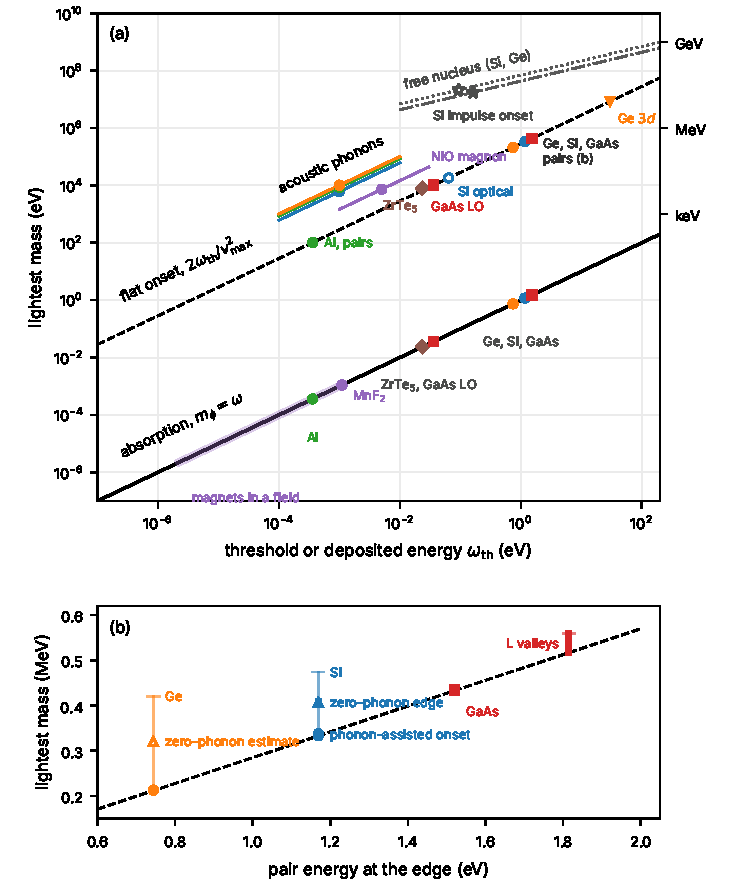
\includegraphics[width=0.78\linewidth]{figures/ch09/fig9_1.pdf}
  \caption{The kinematic map at $v_{\mathrm{max}} = \SI{794.5}{km.s^{-1}}$ (\cref{tab:1-shm}), elastic scattering. (a)~Lightest dark-matter mass of each scattering channel and lightest absorbed boson mass, against the threshold or the energy of the excitation. Solid black: absorption, $m_\phi = \omega$. Dashed: the floor $2\omega_{\mathrm{th}}/v_{\mathrm{max}}^2$, reached by flat onsets. Colored lines: acoustic edges $\omega_{\mathrm{th}}/[2c_\nu(v_{\mathrm{max}} - c_\nu)]$ for the fastest longitudinal speeds of silicon (\SI{9.35}{km.s^{-1}}, lowest), aluminum (\SI{6.67}{km.s^{-1}}, along [111]) and germanium (\SI{5.60}{km.s^{-1}}), drawn from 0.1 to \SI{10}{meV}, with their values at \SI{1}{meV} (dots); purple, the magnon edge of NiO with $c_{\mathrm{M}} = 1.36\times10^{-4}$, with its value at \SI{5}{meV}. Gray: largest free recoil of a silicon (dash-dotted) and germanium (dotted) nucleus, with the impulse onsets (stars; open: estimate). Points on the floor: aluminum pair breaking, the optical phonons of GaAs (square) and silicon (open circle), the germanium $3d$ shell; diamond and bar: ZrTe$_5$, isotropic cone and principal axes (the lowest end, \SI{7.1}{keV}, is its lightest mass). Points on the absorption line: aluminum, MnF$_2$, ZrTe$_5$, GaAs (optical phonon), germanium, silicon and GaAs (electrons); band: the uniform mode of a magnet tuned by a field. (b)~Electron--hole pairs. Filled circles and squares: phonon-assisted onsets; thick bars and filled triangle: zero-phonon edges (silicon, GaAs L valleys); open triangle: germanium zero-phonon estimate, which bounds the edge in neither direction; thin lines: from the floor to the mass that deposits the gap at exactly the valley momentum. Values and their sources in \cref{tab:9-edges}.}
  \label{fig:9-kinmap}
\end{figure}

\begin{table}[tbp]
  \caption{Channel edges of five targets: the lightest mass that reaches each channel in elastic scattering, and the lightest absorbed boson mass, at $v_{\mathrm{max}} = \SI{794.5}{km.s^{-1}}$. Masses in MeV unless marked. ``--'': no such channel; ``n.e.'': not evaluated in this book. The last column gives the section where each value is computed. Entries without a section there are computed here from \cref{eq:9.2-mch}: the aluminum acoustic edge, with the speed \SI{6.67}{km.s^{-1}} along [111] from the zero-temperature elastic constants and density of \cref{sec:20.3}; the floor of ZrTe$_5$; and the silicon $2p$ edge. Estimates are marked.}
  \label{tab:9-edges}
  \centering\footnotesize\setlength{\tabcolsep}{2.5pt}
  \begin{tabular}{@{}>{\raggedright\arraybackslash}p{0.18\linewidth}>{\raggedright\arraybackslash}p{0.12\linewidth}>{\raggedright\arraybackslash}p{0.12\linewidth}>{\raggedright\arraybackslash}p{0.13\linewidth}>{\raggedright\arraybackslash}p{0.08\linewidth}>{\raggedright\arraybackslash}p{0.12\linewidth}>{\raggedright\arraybackslash}p{0.10\linewidth}@{}}
    \toprule
    Channel & Si & Ge & GaAs & Al & ZrTe$_5$ & Section \\
    \midrule
    Floor of the gap, $2\Eg/v_{\mathrm{max}}^2$ & 0.333 & 0.212 & 0.433 & -- & \SI{6.72}{keV} ($4\Delta_{\mathrm{D}}/v_{\mathrm{max}}^2$) & \cref{sec:1.3} \\
    Pairs with a phonon (onset) & 0.3332 (exciton), 0.3374 (free pair) & 0.2119--0.2141 & 0.433--0.436 & -- & n.e. & \cref{sec:13.1} \\
    Pairs without a phonon & 0.405--0.408 & $\approx 0.32$; estimate & 0.517--0.560 (L valleys) & -- & \SI{7.1}{keV} (slow axis; 9.0, \SI{9.6}{keV} along the others) & \cref{sec:13.9,sec:13.1,sec:16.1} \\
    Pair breaking, $2\Delta_{\mathrm{BCS}}$ & -- & -- & -- & \SI{0.10}{keV} & -- & \cref{sec:7.2} \\
    One acoustic phonon, $\omega_{\mathrm{th}} = \SI{1}{meV}$ & \SI{6.1}{keV} & \SI{10.2}{keV} & 10.3--\SI{12.3}{keV} (computed tensors) & \SI{8.6}{keV} & n.e. & \cref{sec:11.1,sec:17.1,sec:17.6} \\
    One optical phonon & \SI{18.3}{keV} & n.e. & \SI{10.35}{keV} & -- & n.e. & \cref{sec:17.3,sec:11.2} \\
    Core shell & 28.6 ($2p$) & 8.5--8.7 ($3d$) & n.e. & n.e. & n.e. & \cref{sec:10.6} \\
    Free nuclear recoil (impulse onset) & 17.5 & 21.3; estimate & n.e. & n.e. & n.e. & \cref{sec:11.4,sec:17.1} \\
    Absorption, lowest $m_\phi$ & \SI{1.1728}{eV} (pairs with a phonon) & $\approx\SI{0.74}{eV}$ with a phonon, \SI{0.89}{eV} without & \SI{36.35}{meV} (optical phonon); \SI{1.52}{eV} (pairs) & \SI{0.36}{meV} & \SI{23.6}{meV} & \cref{sec:13.8,sec:3.3,sec:11.8,sec:15.4,sec:16.1} \\
    \bottomrule
  \end{tabular}
\end{table}

Inside the first group the map orders the targets by stiffness and by gap. At a common threshold of \SI{1}{meV} the acoustic edge falls as the longitudinal sound speed rises, from \SI{6.1}{keV} in silicon to 10.3 to \SI{12.3}{keV} in GaAs, whose elastic tensor is a computed one (\cref{tab:9-edges}; \cref{sec:17.6}, which ranks the targets when their inputs are uncertain). Diamond reaches \SI{3.1}{keV} (\cref{sec:17.5}, figures of merit of the channels). A flat mode competes with an acoustic one read out at a much lower threshold. The optical phonon of GaAs at \SI{36.35}{meV} opens at \SI{10.35}{keV}, the acoustic edge that silicon has at a threshold of \SI{1.7}{meV}. The pairs of ZrTe$_5$ across \SI{23.6}{meV} open at \SI{7.1}{keV}, the silicon edge at \SI{1.16}{meV}; and the NiO magnon at \SI{5}{meV} opens at \SI{7.3}{keV}, the silicon edge at \SI{1.2}{meV}.

In the second group the gap sets the order, germanium, silicon and GaAs, and every crystal of the three has a band above its floor in which pairs need a phonon. In germanium the upper end of that band is not known, and in GaAs it ends where the L valleys open. A detector that counts pairs reaches its floor through phonon-assisted scattering, the process that \cref{chap:13} treats. In the third group the square-root growth of the free-recoil mass makes the nuclear edge of germanium higher than that of silicon by only $(M_{\mathrm{Ge}}/M_{\mathrm{Si}})^{1/2}$ at equal recoil energy.

The map ranks reach, not rate. At the edge itself only particles at $v_{\mathrm{max}}$, moving along the right direction, contribute, and the rate vanishes (\cref{sec:1.3-edge}); a reach curve turns up steeply as the mass approaches the edge from above. For one acoustic phonon, \cref{sec:11.1} finds that the rate comes within \SI{10}{\percent} of its value for heavy particles only above 44 times the edge. Comparing two targets near their edges therefore needs the rates of the chapters that follow.

\begin{workedexample}{The acoustic edge of silicon at a threshold of 1 meV}\label{we:9-acoustic}
The fastest longitudinal branch of silicon runs along $[111]$, with $c_{\mathrm{LA}} = \SI{9.35}{km.s^{-1}}$ from the measured elastic constants (\cref{we:5-debye}). In units of the speed of light, $c_{\mathrm{LA}} = 9.35/299792 = 3.119\times10^{-5}$, and $v_{\mathrm{max}} = 794.5/299792 = 2.650\times10^{-3}$. A phonon of energy $\omega_{\mathrm{th}} = \SI{1}{meV}$ on this branch carries
\begin{equation*}
  \bar q = \frac{\omega_{\mathrm{th}}}{c_{\mathrm{LA}}} = \frac{\SI{e-3}{eV}}{3.119\times10^{-5}} = \SI{32.1}{eV} .
\end{equation*}
This is $0.014\,(2\pi/a)$, with $2\pi/a = \SI{2.28}{keV}$, deep in the linear part of the branch, where the edge needs slopes that obey the acoustic sum rule (\cref{sec:5.2}). With $v_{\mathrm{max}} - c_{\mathrm{LA}} = 2.619\times10^{-3}$,
\begin{equation*}
  m_{\mathrm{min}}^{\mathrm{ac}} = \frac{\SI{e-3}{eV}}{2 \times 3.119\times10^{-5} \times 2.619\times10^{-3}} = \SI{6.12}{keV} .
\end{equation*}
The floor at the same threshold is $2\omega_{\mathrm{th}}/v_{\mathrm{max}}^2 = \SI{0.285}{keV}$. A particle of \SI{6.12}{keV} at $v_{\mathrm{max}}$ has \SI{21.5}{meV} of kinetic energy and could give all of it to a target that absorbs the momentum $\mchi v_{\mathrm{max}} = \SI{16.2}{eV}$, but a phonon with that momentum carries only \SI{0.51}{meV}. To create the \SI{1}{meV} phonon the particle must reverse its direction, giving $2\mchi(v_{\mathrm{max}} - c_{\mathrm{LA}}) = \SI{32.1}{eV}$, and it keeps \SI{20.5}{meV} of its energy. Along $[100]$ the transverse speed \SI{5.84}{km.s^{-1}} of \cref{we:5-debye} would give \SI{9.76}{keV}, but a transverse phonon along a symmetry axis carries no density and is not excited by a density coupling. The edge scales linearly with the threshold, \SI{0.61}{keV} at \SI{0.1}{meV} and \SI{61}{keV} at \SI{10}{meV}, as long as $\bar q$ stays in the linear part of the branch; at \SI{10}{meV} it is already $0.14\,(2\pi/a)$. \Cref{sec:11.1} evaluates the rate near this edge with all branches and directions.
\end{workedexample}

\subsection{Dependence on the halo}\label{sec:9.2-halo}

Every scattering edge moves with $v_{\mathrm{max}} = v_{\mathrm{esc}} + v_{\mathrm{E}}^{\mathrm{ref}}$, but not by the same amount. At the minimum of \cref{eq:9.2-mch} either the derivative with respect to $q$ vanishes or $q$ sits on a constraint that does not depend on $v_{\mathrm{max}}$. Differentiating then leaves the explicit dependence alone:
\begin{equation}
  \frac{\dd\ln m_{\mathrm{min}}^{\mathrm{ch}}}{\dd\ln v_{\mathrm{max}}} = -\frac{\bar qv_{\mathrm{max}}}{\bar qv_{\mathrm{max}} - E_{\mathrm{ch}}(\bar q)} .
  \label{eq:9.2-halo}
\end{equation}
The ratio on the right compares the largest energy the particle could deposit at $\bar q$ with what is left after the excitation is paid. For a flat onset $\bar q = 2E_0/v_{\mathrm{max}}$, half of $\bar qv_{\mathrm{max}}$ goes into the excitation, and the exponent is $-2$, the halo dependence of the floor in \cref{sec:1.3}. For a gapless linear branch $\bar q = \omega_{\mathrm{th}}/c_{\mathrm{ch}}$ and the exponent is $-v_{\mathrm{max}}/(v_{\mathrm{max}} - c_{\mathrm{ch}})$, which is $-1.012$ for silicon: the acoustic edge scales as $1/v_{\mathrm{max}}$, not $1/v_{\mathrm{max}}^2$, because the excitation takes the small fraction $c_\nu/v_{\mathrm{max}}$ of $\bar qv_{\mathrm{max}}$. A free nucleus gives $-1$ for $\mchi \ll M$, from $\mchi \simeq (M\omega_{\mathrm{th}}/2)^{1/2}/v_{\mathrm{max}}$. At a stationary minimum, where the derivative with respect to $q$ vanishes, $\bar qv_{\mathrm{max}} = 2E_{\mathrm{ch}} - \bar qE_{\mathrm{ch}}'$. A branch that rises there takes more than half of $\bar qv_{\mathrm{max}}$, and the exponent exceeds 2 in magnitude: $-2.37$ for the isotropic cone of ZrTe$_5$, and $-2.12$ to $-2.74$ along its axes. A branch that falls there, as on the way to an indirect valley, gives less than 2. The gapless linear branch also rises, but its minimum sits on the constraint $q \ge \omega_{\mathrm{th}}/c_{\mathrm{ch}}$, not at a stationary point. Absorption, \cref{eq:9.2-abs}, does not depend on the halo at all.

The halo matters at the level of a few percent. The uncertainty of \SI{25}{km.s^{-1}} in the escape speed moves the floor and every flat onset by \SI{6.3}{\percent} (\cref{sec:1.3}; exactly \SI{-6.0}{\percent} and \SI{+6.6}{\percent}), and to first order the acoustic edge of silicon by \SI{3.2}{\percent}, the free-recoil edges by \SI{3.1}{\percent} and the Dirac edge of ZrTe$_5$ by \SI{7.4}{\percent}. Over the year the acoustic edge of silicon moves by \SI{-2.0}{\percent} in June and \SI{+1.7}{\percent} in December, about half the shift of the floor. A different halo thus shifts the map without reordering channels of the same shape, but it changes the ratio between a flat and a linear edge by about $\delta\ln v_{\mathrm{max}}$. \Cref{sec:17.3}, which treats inelastic scattering into collective modes, finds that a splitting of \SI{10}{meV} moves the phonon and magnon edges by 12 to \SI{28}{\percent} and the electronic edge of silicon by \SI{1}{\percent} (\cref{tab:17-endo}). An exothermic splitting larger than the excitation energy removes the edge altogether, as \cref{sec:1.3} found for the threshold mass.

\section{Excitations on the momentum--energy plane}\label{sec:9.3}

At $q = \SI{50}{keV}$ and $\omega = \SI{50}{meV}$ silicon has phonon final states and nothing else. At \SI{1}{keV} and \SI{1.3}{eV} its one final state is an electron--hole pair together with a phonon; at \SI{1}{keV} and \SI{3}{eV} a pair without a phonon is open as well. Each excitation in the atlas of \cref{tab:9-atlas} has a \emph{support}, the region of the $(q,\omega)$ plane where its response $S(\vect{q},\omega)$ of \cref{sec:4.2} carries weight. Where the support is formally unbounded, as for the multiphonon tails of \cref{sec:5.6}, we draw the region that holds \SI{90}{\percent} of the weight. \Cref{fig:9-qomega} draws the supports of silicon on the axes of \cref{fig:1-kinematics}, each in the color of its sector of \cref{eq:8.6-partition}. Where two supports overlap, a rate can count a final state twice, or drop an interference term, and the decomposition theorem of \cref{sec:8.6} decides which of the two dangers is real.

\subsection{The silicon plane by sector}\label{sec:9.3-silicon}

\begin{figure}[tbp]
  \centering
  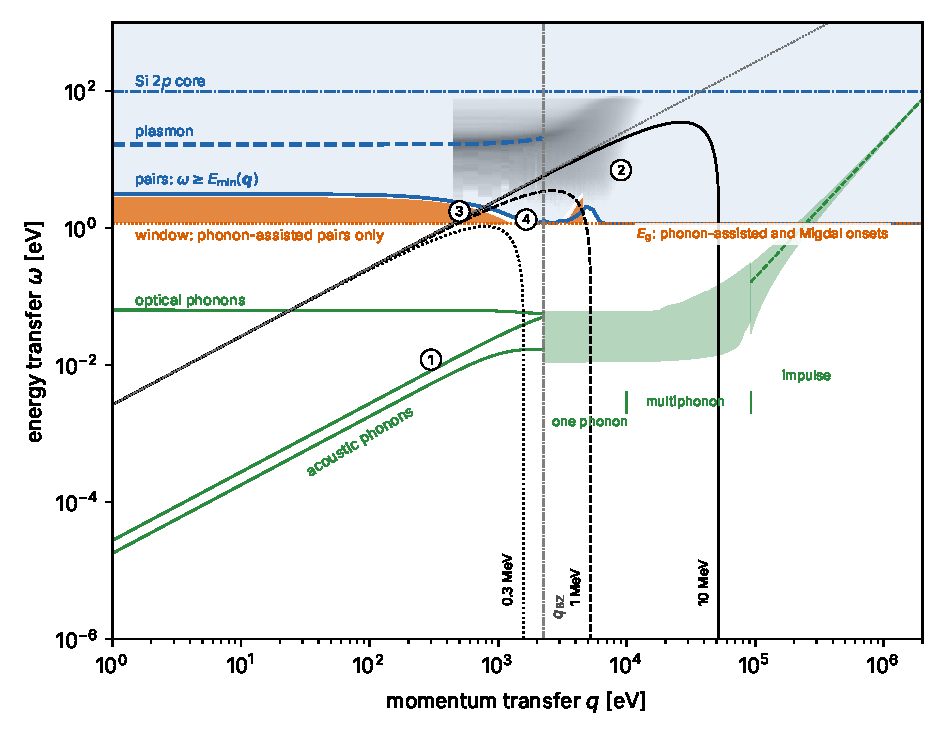
\includegraphics[width=\linewidth]{figures/ch09/fig9_2.pdf}
  \caption{The excitations of silicon on the plane of momentum transfer $q$ and energy deposited $\omega$, on the axes of \cref{fig:1-kinematics}. Green, electron-following sector: the transverse and longitudinal acoustic branches and the optical branch along [100] inside the zone, from the PBE force constants of \cref{sec:5.2}; beyond the zone radius $q_{\mathrm{BZ}} = \SI{2.25}{keV}$ (dash-dotted), the band holding the central \SI{90}{\percent} of the weight that creates phonons (5 and \SI{95}{\percent} quantiles), in the incoherent harmonic response at $T = 0$ with the PBE density of states, and above \SI{92.5}{keV} the same quantiles of the impulse Gaussian about the free recoil $q^2/2M$ (dashed); ticks at \SI{10}{keV} and \SI{92.5}{keV} separate the one-phonon, multiphonon and impulse regimes. Blue, zero-phonon electronic sector: the pair continuum above $E_{\mathrm{min}}(\vect{q})$, drawn as the lowest of the PBE edges along [100], [110] and [111] with the conduction bands shifted to the measured gap $\Eg = \SI{1.17}{eV}$, and as $\Eg$ beyond \SI{6.5}{keV}; gray scale, the random-phase loss function with local fields of the tables of Knapen, Kozaczuk and Lin~\cite{knapen2021dark} (scissor to the gap of \SI{1.17}{eV}, directions averaged, \num{e-3} to 4 on a logarithmic scale); dashed, the plasmon of the valence electron gas, $\omega_{\mathrm{pl}}^2 = \omega_p^2 + \tfrac35q^2v_{\mathrm{F}}^2$ with $\omega_p = \SI{16.6}{eV}$, up to \SI{2.24}{keV}, where this dispersion meets the pair continuum; dash-dotted, the $2p$ core level at \SI{99.4}{eV}. Orange, phonon-dressed electronic sector: the off-shell window along [100], from the phonon-assisted onset $\Eg + \omega_{\mathrm{TA}}$ up to $E_{\mathrm{min}} - \delta_{\mathrm{w}}$ with $\delta_{\mathrm{w}} = \SI{0.3}{eV}$; white above it, the margin of width $\delta_{\mathrm{w}}$ below the edge; dotted, $\Eg$, above which phonon-assisted pairs and Migdal events exist at every $q$. Black: the largest energy deposited, $qv_{\mathrm{max}} - q^2/2\mchi$, for $\mchi = 0.3$ (dotted), 1 (dashed) and \SI{10}{MeV} (solid), and $qv_{\mathrm{max}}$ (gray dotted), with $v_{\mathrm{max}} = 2.650\times10^{-3}$. Circled numbers mark the interference terms of \cref{tab:9-overlaps}.}
  \label{fig:9-qomega}
\end{figure}

\paragraph{Electron-following sector.} Inside the zone the support is a set of lines, the phonon branches of \cref{sec:5.2}. The acoustic branches rise as $\omega = c_\nu q$ from the origin and flatten at the zone boundary, at \SI{17}{meV} (transverse) and \SI{51}{meV} (longitudinal) at X in the PBE calculation; the optical branch stays near \SI{64}{meV}. Beyond the zone nothing new appears in energy. The momentum transfer is never folded (\cref{sec:1.3}); the nucleus keeps $\vect{q}$, and the phonon carries $\vect{q}$ minus a reciprocal-lattice vector. A single phonon therefore has energies between zero and \SI{64}{meV} at every $q$, and its weight changes as the Debye--Waller exponent $2W_\kappa = q^2\langle u_x^2\rangle$ of \cref{eq:5.6-W} grows. The PBE density of states of \cref{sec:5.2} gives $\langle u_x^2\rangle = \SI{2.45e-3}{\angstrom^2}$ at $T = 0$, so $2W_\kappa = 0.016$ at \SI{5}{keV}, 0.063 at \SI{10}{keV} and 1.0 at \SI{40}{keV}. Two and more phonons fill the band as $2W_\kappa$ approaches one. In the incoherent approximation the central \SI{90}{\percent} of the weight that creates phonons lies between 11 and \SI{60}{meV} at the zone radius $q_{\mathrm{BZ}} = \SI{2.25}{keV}$, still the one-phonon band. It lies between 13 and \SI{129}{meV} at \SI{46}{keV}, where the recoil parameter $x_R$ of \cref{eq:8.5-xR} is one, and between 46 and \SI{311}{meV} at \SI{92.5}{keV}. At that momentum the impulse approximation of \cref{sec:11.4} takes over from the sum over phonon numbers. It treats the nucleus as kicked so hard that its spectrum is a Gaussian of width $(E_R\langle\omega\rangle)^{1/2}$ about the free recoil energy $E_R = q^2/2M$, with $\langle\omega\rangle = \SI{40.9}{meV}$ the mean phonon energy. From there on the support is a band that follows $q^2/2M$ and narrows in relative width as $x_R^{-1/2}$.

The free recoil line crosses the gap at $q = (2M\Eg)^{1/2} = \SI{247}{keV}$, and the upper edge of the band does so at \SI{212}{keV}. Above these momenta electron-following final states sit at the same $(q,\omega)$ as electronic ones. A particle must be heavier than \SI{46.8}{MeV} to supply \SI{247}{keV}.

\paragraph{Zero-phonon electronic sector.} An electron--hole pair with no net phonon must take the whole momentum transfer itself, and its support is the continuum $\omega \ge E_{\mathrm{min}}(\vect{q})$ of \cref{eq:3.3-Emin}. With the bands of \cref{fig:3-si-bands}, shifted to the measured indirect gap, the edge lies at \SI{3.17}{eV} for $q \to 0$, at \SI{1.77}{eV} at \SI{1}{keV} along the lowest of the three symmetry directions, and reaches $\Eg = \SI{1.17}{eV}$ at the valley momentum $k_{\mathrm{c}} = \SI{1.94}{keV}$. The value at $q \to 0$ lies below the measured direct gap of \SI{3.4}{eV}, because a shift fitted to the indirect gap does not correct the vertical gap at $\mathrm{\Gamma}$ (\cref{sec:3.3}). At larger $|\vect{q}|$ the edge depends on the direction of $\vect{q}$. It returns to $\Eg$ whenever $\vect{q}$ equals a valley momentum plus a reciprocal-lattice vector, $\vect{k}_{\mathrm{c}} + \vect{G}$, whose lengths are 1.94, 2.63, 3.25, 4.96, 5.27, \SI{5.32}{keV} and so on. Above \SI{6.4}{keV} they leave no gap wider than \SI{0.72}{keV}, and half that distance costs a pair of mass $1.19\,m_e$ about \SI{0.11}{eV} above $\Eg$. There the onset of the direction average that enters an isotropic rate stays within about a tenth of an eV of the gap. Below, the widest gap lies between 3.25 and \SI{4.96}{keV}; there the lowest of the three symmetry-line edges rises to \SI{2.07}{eV}, an upper value for the onset over all directions. Upward the continuum is unbounded. At small $q$ its weight sits at the absorption peaks of 3.4 and \SI{4.2}{eV} and in the plasmon; at large $q$ it concentrates along the free-electron recoil $q^2/2m_e$, the ridge of the gray scale in \cref{fig:9-qomega}.

The plasmon, the exciton and the core shells lie inside this region and have homes of their own. The plasmon of \cref{sec:4.5} starts at the measured loss peak of \SI{16.4}{eV}, \SI{0.2}{eV} below the $\omega_p = \SI{16.6}{eV}$ of the valence electron gas, and disperses upward. With the quadratic dispersion of the gas it is a line up to \SI{2.24}{keV}, where it enters the pair continuum and Landau damping removes its weight; the exact zero of the Lindhard function enters at $q_{\mathrm{c}} = \SI{2.60}{keV}$ (\cref{sec:4.5}). In the loss-function tables that \cref{sec:10.2} uses, the peak moves from \SI{18.9}{eV} at \SI{0.5}{keV} to \SI{22.3}{eV} at \SI{2.45}{keV}; the small-$q$ peak lies \SI{2.5}{eV} above the measured \SI{16.4}{eV} because of the shift that sets their gap (\cref{sec:10.3}, which computes the plasmon's share of the rate). The bound pair, the exciton of \cref{sec:4.9}, lies \SI{14.7}{meV} below the edge near $q = k_{\mathrm{c}}$; on the scale of the figure it coincides with the edge (\cref{sec:10.5}, the exciton lines at finite momentum). The core shells start at fixed energies, \SI{99.4}{eV} for $2p$ and \SI{150}{eV} for $2s$, and carry weight at momentum transfers of tens of keV, the momenta of the electrons in them (\cref{sec:10.6}).

\paragraph{Phonon-dressed electronic sector.} A pair created together with a phonon needs no particular momentum, because the phonon carries whatever crystal momentum the pair lacks. Its support starts just above the gap at every $q$, at the onset $E^{\mathrm{PA}}_{\mathrm{min}}(\vect{q}) = \Eg + \omega_{\mathrm{TA}}(\vect{k}_{\mathrm{c}} - \vect{q})$ of \cref{eq:13.1-EPA}, and never above $\Eg + \SI{64}{meV} = \SI{1.23}{eV}$. With the PBE force constants the onset is \SI{1.187}{eV} at $q \to 0$ and \SI{1.184}{eV} at \SI{1}{keV}. Between this onset and the zero-phonon edge lies the \emph{off-shell window} of \cref{sec:8.6}, the region below $E_{\mathrm{min}}(\vect{q}) - \delta_{\mathrm{w}}$ where no zero-phonon pair exists and every electronic final state carries a phonon. Along the valley axis, with $\delta_{\mathrm{w}} = \SI{0.3}{eV}$, it spans 1.184 to \SI{1.467}{eV} at \SI{1}{keV} and closes at \SI{1.27}{keV} with the computed bands. It reopens beyond \SI{3.30}{keV}, on the far side of the Umklapp image of the opposite valley (\cref{sec:13.6}, which fixes the margin and the window edges). Above the zero-phonon edge the same sector is the phonon sideband of the zero-phonon continuum, and there it is a correction to the zero-phonon rate (\cref{sec:13.9} compares the two).

The Migdal effect of a nucleon coupling, which straddles the two electronic sectors (\cref{sec:9.1-sectors}), has the same support. The struck nucleus absorbs the momentum and the electrons take an energy $\omega_e \ge \Eg$, at every $q$. What separates it from a pair made through the electron density is the operator, not the region of the plane.

\subsection{Overlap regions and interference}\label{sec:9.3-overlap}

One phonon and two phonons share the band below \SI{64}{meV}. The impulse band and the pair continuum share the region above \SI{212}{keV} and \SI{1.17}{eV}, and the phonon sideband and the zero-phonon continuum share everything above $E_{\mathrm{min}}(\vect{q})$. An overlap in the plane is not by itself an interference. Sectors add (\cref{sec:9.1-sectors}), to the accuracy of the leak in \cref{eq:8.6-decomp}, and within one sector so do different phonon numbers: one and two phonons are orthogonal final states, and so are a nucleus recoiling with the electrons in their ground state and a pair. Interference needs two amplitudes into the same final state, and on the silicon plane that happens in two ways. The first is a coupling to both species, as for a dark photon, whose cross terms $S_{e\kappa}$ fill the bottom row of \cref{tab:8-sectors} and are derived, with their sizes, in \cref{sec:17.4}. The second is the boundary between the two electronic sectors, within $\delta_{\mathrm{w}}$ below the zero-phonon edge and a few pair widths above it. Only the sum $S^0 + S^+$ is defined there, the Dyson convention \cref{eq:8.6-dyson} splits it, and the decay of a zero-phonon pair can interfere with the same one-phonon state made directly, the Fano term \cref{eq:8.6-fano}. Inside that margin only totals of the two electronic sectors are quoted (\cref{sec:13.6}).

\subsection{The kinematic reach on the plane}\label{sec:9.3-reach}

Particles of mass $\mchi$ reach the region below $\omega = qv_{\mathrm{max}} - q^2/2\mchi$ (\cref{eq:1.3-region}), and the black curves of \cref{fig:9-qomega} show it for three masses. A particle of \SI{0.3}{MeV} deposits at most \SI{1.05}{eV}, at $q = \SI{0.80}{keV}$, and transfers at most \SI{1.59}{keV}. Its region lies below the gap and inside the zone, so it meets single acoustic and optical phonons and nothing else, with $2W_\kappa \le 0.002$. A particle of \SI{1}{MeV} deposits at most \SI{3.51}{eV} and crosses the gap for momentum transfers between 0.49 and \SI{4.81}{keV}. It enters the off-shell window, where every pair it makes carries a phonon, and the zero-phonon continuum above the edge, while its lattice final states are still single phonons ($2W_\kappa \le 0.018$ at its largest $q$, \SI{5.3}{keV}). A particle of \SI{10}{MeV} transfers up to \SI{53}{keV}, where $2W_\kappa = 1.8$, and reaches deep into the multiphonon band. In energy it reaches \SI{35}{eV}, across the region of the plasmon, but not the plasmon line, which ends at \SI{2.24}{keV}, where this particle deposits no more than \SI{5.9}{eV}; nor the $2p$ shell at \SI{99.4}{eV}, nor the impulse band, which opens at \SI{17.5}{MeV}. The lightest mass whose curve touches a region is the lightest mass of that channel (\cref{sec:9.2}).

\begin{workedexample}{The excitations open at 5 keV and 2 eV in silicon}\label{we:9-open}
Take $q = |\vect{q}| = \SI{5}{keV}$ and $\omega = \SI{2}{eV}$. The point is reachable if $qv_{\mathrm{max}} - q^2/2\mchi \ge \omega$, with $qv_{\mathrm{max}} = \SI{13.25}{eV}$, that is for $\mchi \ge q^2/[2(qv_{\mathrm{max}} - \omega)] = \SI{1.11}{MeV}$; at \SI{10}{MeV} the minimum speed of \cref{eq:1.3-vmin} is $\vmin = \omega/q + q/2\mchi = 6.50\times10^{-4}$, or \SI{195}{km.s^{-1}}, well inside the halo.

\emph{Electron-following.} At \SI{5}{keV}, $2W_\kappa = 0.016$ and $E_R = \SI{0.48}{meV}$. Two electronvolts would take at least 32 phonons of \SI{64}{meV}, each costing a factor of order $2W_\kappa$ in weight. The sector is closed.

\emph{Zero-phonon electronic.} The edge depends on the direction of $\vect{q}$. Along [100], [110] and [111] it lies at 2.59, 2.02 and \SI{2.31}{eV}, all above \SI{2}{eV}: along the symmetry lines no pair without a phonon exists at this point. But a valley image $\vect{k}_{\mathrm{c}} + \vect{G}$ has length \SI{4.96}{keV}, and for $\vect{q}$ near that direction the pair costs $\Eg$ plus about \SI{1}{meV}. Averaged over directions the zero-phonon response is thus open, but small: the direction-averaged loss function of the tables of \cref{sec:10.2} at this $q$ is \num{8.8e-4} at \SI{2}{eV}, against its maximum of 0.33 at \SI{35.7}{eV}. The plasmon line has ended at \SI{2.24}{keV}, the exciton lies \SI{14.7}{meV} below the edge, and the $2p$ shell needs \SI{99.4}{eV}: none of them is open.

\emph{Phonon-dressed electronic.} The phonon-assisted onset lies below \SI{1.23}{eV} for every $\vect{q}$, so phonon-assisted pairs are open. Where the point sits relative to the zero-phonon edge again depends on direction. Along [100] it lies below $E_{\mathrm{min}} - \delta_{\mathrm{w}} = \SI{2.29}{eV}$, inside the window, and phonon-assisted pairs are the one electronic final state there. Along [111] it lies inside the window by \SI{11}{meV} ($E_{\mathrm{min}} - \delta_{\mathrm{w}} = \SI{2.011}{eV}$), less than the exciton binding and less than the difference between a symmetry-line edge and the minimum over all crystal momenta. Along [110] it lies in the margin, between 1.72 and \SI{2.02}{eV}, where only the total of the two electronic sectors is defined. A nucleon coupling reaches the same final states through the Migdal effect, with a probability per scattering of order $(E_R/\langle\omega_e\rangle)(\delta M_\kappa/M_\kappa) = 2\times10^{-8}$ by the moment estimate of \cref{sec:12.1}. Here $\langle\omega_e\rangle \approx \SI{6}{eV}$ is the mean electronic excitation energy, and $\delta M_\kappa/M_\kappa = Z_\kappa m_e/M_\kappa = 2.7\times10^{-4}$ the share of the atom's mass carried by the electrons that move with the nucleus (\cref{sec:8.6}).

\emph{Interference.} For a dark photon the cross cells of regions 2 and 3 of \cref{tab:9-overlaps} are both present, each a few parts in $10^4$ of its sector, and for directions in the margin the Fano term of region 4 vanishes in silicon. The point is thus served by two sectors in different directions of $\vect{q}$, which is why a calculation applies the window bin by bin in $(|\vect{q}|,\hat{\vect{q}})$ and not to the direction average (\cref{sec:13.6}).
\end{workedexample}

\subsection{Supports in other materials}\label{sec:9.3-others}

The remaining rows of the atlas belong to other materials, and their supports reduce to a few shapes: a dispersing line, a flat line at a fixed energy, a continuum above a threshold, or a point at $q \to 0$. \Cref{tab:9-supports} gives the shape and one number for each, with the section that treats it. Absorption samples the single point of \cref{eq:9.2-abs}, far to the left of every scattering curve, and a support absorbs if it reaches $q \to 0$ at that energy (\cref{sec:9.1-empty}).

\begin{table}[tbp]
  \centering
  \small
  \caption{Supports in the $(q,\omega)$ plane of the excitations of the atlas that silicon does not have, with one characteristic number for the material that the treating section uses. ``Line'' means one energy for each $q$; ``continuum'' a band of energies at each $q$. $g_{33}$: component of the gyration tensor along the optic axis; $g_c$: Luttinger charge parameter of a one-dimensional metal.}
  \label{tab:9-supports}
  \begin{tabular}{@{}p{0.24\linewidth}p{0.32\linewidth}p{0.23\linewidth}p{0.10\linewidth}@{}}
    \toprule
    Excitation & Support & Scale & Home \\
    \midrule
    Optical phonons of polar crystals & line at $\omega_{\mathrm{L}}$ as $q \to 0$, reached by a coupling to charge & GaAs \SI{36.35}{meV} & \cref{sec:11.2} \\
    Phonons of a quantum crystal & acoustic lines and multiphonon band of a light, strongly anharmonic lattice & solid helium, below \SI{3}{meV} at low pressure & \cref{sec:11.5} \\
    Magnons & line from an anisotropy gap at the zone center to the top of the band & NiO, gap \SI{4.54}{meV} (measured; anisotropy added to the model), top \SI{118}{meV} & \cref{sec:14.1} \\
    Two-magnon continua & continuum from the one-magnon energy to twice the band top at small $q$ & NiO, up to \SI{236}{meV} & \cref{sec:14.2} \\
    Chiral and nonreciprocal modes & the supports above; the response acquires a part odd in $\vect{q}$ & $\alpha$-quartz, $q\,g_{33} = 7\times10^{-5}$ at \SI{2.1}{eV} & \cref{sec:14.5} \\
    Precessing nuclear spins & point at $q \to 0$, $\omega$ at the Larmor frequency & $^{207}$Pb in \SI{26.8}{mT}: \SI{241.8}{kHz} (\SI{1}{neV}) & \cref{sec:14.6} \\
    Superconducting quasiparticle pairs & continuum $\omega \ge 2\Delta_{\mathrm{BCS}}$ inside the particle--hole band $\omega \le qv_{\mathrm{F}} + q^2/2m_e$ of the metal & aluminum, $2\Delta_{\mathrm{BCS}} = \SI{0.36}{meV}$ & \cref{sec:15.1} \\
    Dirac and narrow-gap pairs & continuum $\omega \ge (4\Delta_{\mathrm{D}}^2 + v_{\mathrm{D}}^2q^2)^{1/2}$ & ZrTe$_5$, $\Delta_{\mathrm{D}} = \SI{11.8}{meV}$ & \cref{sec:16.1} \\
    Low-dimensional plasmons & line $\omega \propto q_\parallel$, faster than the halo, reached by oblique $\vect{q}$ & metallic nanotube, $\omega = v_{\mathrm{D}}q_\parallel/g_c$, 3.4 to 6.9 times $v_{\mathrm{max}}$ & \cref{sec:16.2} \\
    Graphene, nanotubes, quantum dots & continuum above a confinement gap; ejection above the work function & PbS dot \SI{1.2}{eV}; graphene \SI{4.3}{eV} & \cref{sec:16.3} \\
    Molecular (Frenkel) excitons & nearly flat lines at molecular energies & anthracene \SI{3.1}{eV} & \cref{sec:16.4} \\
    Dopant transitions & flat lines and an ionization continuum & Si:P, binding \SI{45.59}{meV} & \cref{sec:16.5} \\
    Color centers, broken bonds & reached through a nuclear recoil above a displacement or bond energy & H$_2$ bond \SI{4.75}{eV}; displacement tens of eV & \cref{sec:16.6} \\
    Two-level systems in glasses & flat continuum of splittings, independent of $q$ & down to \si{\micro eV}; \SI{e20}{eV^{-1}.cm^{-3}} & \cref{sec:16.7} \\
    Bulk acoustic modes of a body & points at $q \to 0$, the normal modes of the whole detector & MHz (mm crystal) to kHz (ton-scale bar) & \cref{sec:11.8} \\
    \bottomrule
  \end{tabular}
\end{table}

For superconductors and Dirac materials the sectors are those of quasiparticle number (\cref{sec:9.1-sectors}), so the rules of \cref{sec:9.3-overlap} for which overlaps add and which interfere hold only as far as those sectors are defined, which \cref{sec:8.6} bounds but does not settle.

\section{Limit Checks and the truncation label}\label{sec:9.4}

The free-recoil formula $\omega = q^2/2M$ holds for a silicon nucleus once the recoil energy exceeds nine phonon energies, \SI{0.54}{eV} for a nucleus in an Einstein well of \SI{60}{meV}. \Cref{lim:1.3a} showed this with one plot: the formula against the bound nucleus, the recoil energy on the horizontal axis, and a gray band where the two agree. The channel chapters recover 90 published formulas as limits of their own results, and test 80 of them in 75 boxes of the same kind. Each box answers one question: over what range of a single parameter does the published formula agree with a fuller calculation, and what fails outside that range? We build such a box, show that its horizontal axis follows from the place of the formula on the truncation label $\mathfrak{T}$ of \cref{sec:8.5}, and place every formula of \crefrange{chap:10}{chap:17} on that label.

\subsection{The comparison plot}\label{sec:9.4-plot}

A Limit Check has three parts: the formula, a plot, and one sentence. The formula is written in the book's notation, with the symbols of \cref{chap:8}, and a one-line citation names the equation of the source where it was first given.

The plot compares the formula with a fuller result for the same quantity. In the language of \cref{sec:8.8}, the formula is a quantity evaluated at a point $\mathfrak{T}$ of the label and the fuller result is the same quantity one step further along one axis, at $\mathfrak{T}_k^+$; the plot shows their relative difference $\delta_k$ of \cref{eq:8.8-delta}. Most boxes plot the ratio of the two, $1 + \delta_k$ or its inverse, so that the formula is the horizontal line at one. Some plot both curves, when their shapes matter more than their ratio. The fuller result is computed in the book, from a crystal calculation or from a model that keeps the physics the formula drops, or it is measured. In \cref{lim:1.3a} it is the nucleus bound in an Einstein potential, whose spectrum is a series of phonon lines.

The horizontal axis carries the \emph{controlling parameter}, the variable along which $\delta_k$ runs from negligible at one end of the axis to order one at the other. In \cref{lim:1.3a} it is $E_R/\omega_0$, the recoil energy in units of the phonon energy. The \emph{leading correction}, the first term of $\delta_k$ in the controlling parameter, is drawn as a third curve, usually dotted or dashed. In \cref{lim:1.3a} it is the rms width $(E_R\omega_0)^{1/2}$ of the deposit, which falls relative to $E_R$ as $(\omega_0/E_R)^{1/2}$. The gray band marks the values of the controlling parameter at which the formula agrees with the fuller result. The tolerance is stated in the caption: usually \SI{10}{\percent}, sometimes \SI{1}{\percent} or \SI{15}{\percent}, or a fixed fraction of a width, as the rms width below $E_R/3$ that bounds the band of \cref{lim:1.3a}. The caption prints the edge of the band.

The sentence under the plot says what breaks down outside the band, in physical terms: in \cref{lim:1.3a}, that below a few phonon energies the deposit arrives in whole phonons and spreads as widely as $E_R$ itself.

The \emph{approximation chain}, the sequence of steps that leads from the book's general result to the formula, lives in the running text next to the box, where each step is derived or cited to a specific equation. The formal record, with the chain, the conditions, the specification of the plot and the size of the leading correction, is the row of the formula in \cref{tab:F-rows} of \cref{app:F}. How far the book has established the formula is read from what the plot compares with.

Inside the gray band the formula is established to the stated tolerance, relative to the fuller result. That statement is as strong as the fuller result. Where the fuller result is a crystal calculation at a known point of $\mathfrak{T}$, such as the random-phase response with local fields, the band says that the formula agrees with that calculation; the calculation has its own next step, which the label names. Where the fuller result is a model, as the Einstein well of \cref{lim:1.3a} is a model of the silicon lattice, the edge of the band is an estimate of where the formula fails, not a bound. Where nothing is shaded, the formula fails over the whole plotted range, and the box gives the size of the failure instead of a range of validity. Some boxes compare two published forms of one result, or test a sum rule; they are read in the same way, with the exact relation as the fuller result.

\subsection{Placement on the truncation label}\label{sec:9.4-place}

A formula is placed on $\mathfrak{T}$ by reading its assumptions, one component at a time, as \cref{we:8-label} did for phonon-assisted absorption. The eight components of \cref{eq:8.5-label} are five orders and three labels. The orders are those of the Born--Oppenheimer coupling ($n_B$), the electron--phonon vertex ($n_g$), the anharmonicity ($n_A$), the temperature ($n_T$) and the multipole expansion ($n_D$); the labels are the many-body approximation $\mathcal{X}$, the lattice regime $\mathcal{K}$ and the Migdal regime $\mathfrak{M}$. Clamped nuclei put a formula at $n_B = 0$; independent particles at $\mathcal{X} = \mathrm{IP}$; a free nucleus that recoils as a whole at $\mathcal{K}$ = impulse; a kick that the electrons see as instantaneous at $\mathfrak{M}$ = sudden. The deviation notation of \cref{sec:8.5} then lists only the components that differ from the base point $\mathfrak{T}_0$ of \cref{eq:8.5-base}.

The placement fixes the plot. The leading correction of a formula is the largest of its steps $\mathfrak{T} \to \mathfrak{T}_k^+$, and its controlling parameter is whatever makes that step grow. On an axis with a small parameter, the step is a power of the parameter of \cref{tab:8-params}, and the controlling parameter is that small parameter or a variable it grows with. A formula in the impulse regime has the Doppler width as its leading correction, of relative size $x_R^{-1/2}$ by \cref{eq:8.5-width}, so its plot runs against the recoil parameter $x_R$. A Migdal probability at dipole order, $n_D = 2$, misses the higher multipoles, and its plot runs against $\xi_D$. On the many-body axis there is no small parameter (\cref{sec:8.5}). The fuller result is then the next approximation, computed, and the controlling parameter is the variable along which screening changes: the momentum transfer, the energy deposit or the mass of an absorbed boson.

Many formulas truncate an expansion that is not one of the eight components. A long-wavelength form keeps the leading power of $q$ against a lattice momentum, and a light-mediator rate assumes a dark-matter mass far above the kinematic edge. A spin-wave rate keeps the leading order in $1/|\vect{S}|$, and a dopant rate the first order in the donor density. \Cref{sec:8.5} records such approximations as qualifiers, in words, and their controlling parameter is the expansion parameter itself. We sort them into four kinds: long wavelength, as in the plasmon pole of the electron gas; the kinematics of the halo and of the signal, as in a light-mediator rate far above its edge or the coherence time of a classical field; the dark-matter side and the order in the coupling, as in the speed of boosted dark matter; and the model or method used for the target, as in the spin-wave order of a magnon rate or the density of a dopant.

\begin{figure}[tbp]
  \centering
  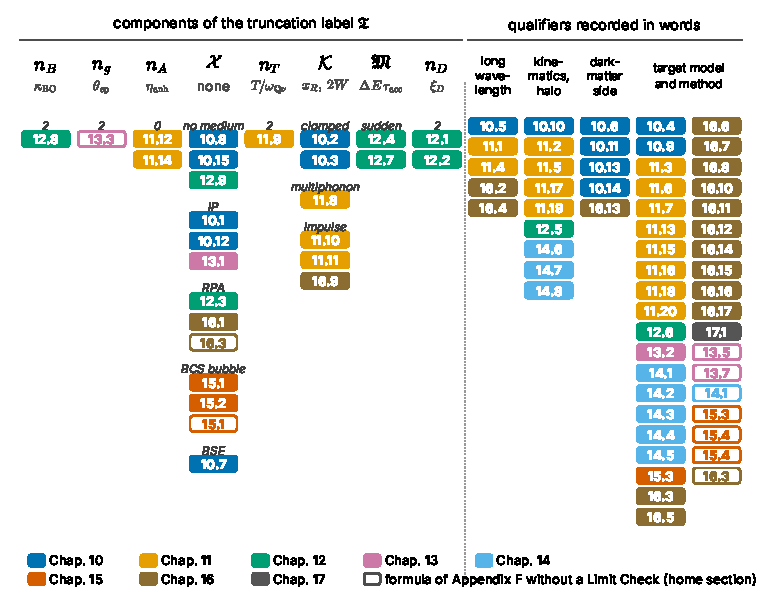
\includegraphics[width=\linewidth]{figures/ch09/fig9_3.pdf}
  \caption{The Limit Checks of \crefrange{chap:10}{chap:17} placed by the axis of their leading correction. Left: the eight components of the truncation label $\mathfrak{T}$, each with its small parameter (\cref{tab:8-params}); under each, the boxes whose comparison result lies one step from the formula along that component, grouped by the formula's value of that component, printed in italic (for example IP or impulse). Right: boxes whose leading correction is an expansion in a parameter that the label records only in words, sorted into four kinds. Filled chips: Limit Checks, colored by chapter. Hollow chips: formulas of \cref{tab:F-rows} without a box, labeled by the number of their home section, not of a box. The step of each box and its controlling parameter are listed in \cref{tab:9-limitchecks}.}
  \label{fig:9-axes}
\end{figure}

\Cref{fig:9-axes} places the 75 Limit Checks of \crefrange{chap:10}{chap:17} by the axis of their leading correction, and \cref{tab:9-limitchecks} lists each with its controlling parameter and its step. Twenty-five lie on a component of the label. Eleven are on the many-body axis. Among them are the crystal form-factor rate of \cref{sec:10.1}, which computes the rate of creating electron--hole pairs from independent-particle bands, and the Migdal rate through the loss function of \cref{sec:12.3}. The loss function of a superconductor in \cref{sec:15.1} is there too: its box compares the bare quasiparticle response with a conserving one, built so that it obeys charge conservation. Six are on the lattice regime, from the clamped lattice to the impulse limit, two on the anharmonic order, two on the Migdal regime, two on the multipole order, one on the thermal order and one on the Born--Oppenheimer order. Every Migdal scattering formula sits at $n_B = 2$, and the rate with phonon final states of \cref{sec:12.4} takes its next step there: the phonon energies in the electronic denominators give $2\langle\omega_{\mathrm{ph}}^2\rangle/\omega_e^2 = 2.9\times10^{-3}$ at the silicon gap, one step of $n_B$ in the counting of \cref{tab:8-params}. None of the boxes has its leading correction on $n_g$. The one formula whose next step is $n_g = 4$, the phonon-assisted electron-recoil rate of \cref{sec:13.3}, has no box, and its correction is the off-shell parameter $\theta_{\mathrm{ep}}$ of \cref{tab:8-params}.

The other 50 boxes expand in a qualifier: 5 in a long wavelength, 9 in the kinematics of the halo or the signal, 5 on the dark-matter side, and 31 in the model of the target. Two of the last are close to the label. Before any change of $\mathcal{X}$, the rate of the electron gas in \cref{sec:10.3} misses the gap and the interband peaks of the crystal, a change of target model. The band of \cref{sec:11.5} built from exact moments misses the skewness of the moment problem, not an anharmonic order. The split follows the chapters. In \cref{chap:12} seven of nine boxes lie on the label, in \cref{chap:10} seven of fifteen and in \cref{chap:11} six of twenty. In \cref{chap:14}, on magnetic excitations, none of the eight does, and in \cref{chap:16}, on novel targets such as Dirac materials, quantum dots and glasses, two of seventeen do. The label was built from the expansion of a crystal of electrons and nuclei in its small parameters, and the electronic, lattice and Migdal channels truncate along it. For the other targets the controlling parameter of the box is the target's own.

\begin{workedexample}{Three literature rates on the truncation label}\label{we:9-place}
We place three rates on $\mathfrak{T}$ and read from each placement the plot that its Limit Check draws. The rates are derived in \cref{sec:10.1,sec:10.2,sec:11.4}; here we use only their assumptions.

\emph{Crystal form-factor rate.} The electron-recoil rate of Essig and collaborators~\cite[Eqs.~(3.13) and (3.17)]{essig2016direct} squares the matrix elements of $\ee^{\ii\vect{q}\cdot\vect{r}}$ between Bloch states of independent electrons (\cref{chap:3}), with the valence bands filled at $T = 0$ and the nuclei clamped. Each assumption is a base value: no derivative coupling, no electron--phonon vertex, independent particles, no thermal occupation, and no multipole expansion, since the plane wave is kept whole. The rate sits at $\mathfrak{T}_0$, with the qualifier ``unscreened''. Every integer step costs a small parameter of \cref{tab:8-params}, and the many-body step costs an amount that no parameter predicts, so the many-body step is computed: IP to RPA to RPA with local fields. Screening is strongest at small $q$, where the long-range Coulomb field of the induced charge acts, and fades at large $q$. The controlling parameter is therefore the momentum transfer at fixed energy, and \cref{lim:10.1a} plots the rate weight against $q/q_0$, with $q_0 = \alpha m_e$, for the three approximations. The screened response is 0.05 of the unscreened one at the kinematic edge and 0.22 at $q_0$, and the $q$-integrated rate at \SI{5}{eV} is 0.47 of it. Nothing is shaded. The status follows: the formula is a definite point of the label, but its leading correction is of order one across the whole range, and \cref{sec:10.2} computes the rate with screening.

\emph{Loss-function rate.} The rate of Knapen and collaborators and of Hochberg and collaborators~\cites[Eqs.~(6) and (13)]{knapen2021dark}[Eq.~(1)]{hochberg2021determining} writes the response through the loss function $\Imag[-1/\varepsilon(\vect{q},\omega)]$. The identity \cref{eq:8.4-exact} makes this form exact for a coupling to the total charge at any lattice and for a coupling to the electron density with the nuclei clamped. The many-body axis is then not truncated by the formula; $\mathcal{X}$ is whatever approximation the loss function is computed in, RPA with local fields in the tables of \cref{sec:10.2}. The truncation is the clamped lattice, for a coupling to electrons alone. Releasing the nuclei is a step of the lattice regime, from no phonon in the final state to one phonon, and it adds the electron-following sector of \cref{sec:8.6}: the electrons that move with a nucleus carry an acoustic peak inside the phonon band. The controlling parameter is the energy deposit against the top of the phonon band, $\omega/\omega_{\max}$, and \cref{lim:10.2a} shades the energies above the band, where the two couplings share the formula. Below it, for dark matter of \SI{1}{MeV} and in a model of the acoustic peak, the electron-only coupling has more than $10^4$ times the rate that electronic excitations give at the same energies. The formula is established above the phonon band; inside it, for an electron-only coupling, the size of the correction rests on a model.

\emph{Free nuclear recoil.} The recoil rate of Lewin and Smith with the Helm form factor~\cite{lewin1996review}, \cref{eq:11.4-LS} with \cref{eq:2.2-helm}, assumes a nucleus that is free, at rest and recoils as a whole. In the label this is $\mathcal{K}$ = impulse at zero width, $n_B = 0$, the same placement as the elastic recoil of \cref{lim:1.3a}. The mean deposit $E_R$ is exact at every anharmonic and thermal order, since it is fixed by the sum rule \cref{eq:5.6-sum}. The leading correction is the next term of the impulse expansion, the Doppler width of the bound nucleus, of relative size $x_R^{-1/2}$. The controlling parameter is $x_R$, and \cref{lim:11.4a} plots the crystal rate over the free-recoil rate against it, with the multiphonon response of silicon as the fuller result and the Gaussian of the impulse approximation as the leading correction. For \SI{1}{GeV} dark matter the two agree within \SI{10}{\percent} for $x_R \ge 2.3$, at $q \ge \SI{70}{keV}$.

The two boxes on the impulse axis draw their bands at different values of one parameter. \Cref{lim:1.3a} asks of the spectrum at one momentum transfer that its rms width be below a third of $E_R$, which needs $x_R \ge 9$ for its oscillator. \Cref{lim:11.4a} asks of the rate at a given energy, which sums the response over momentum transfers with a smooth halo weight, that it agree within \SI{10}{\percent}. That is met at smaller $x_R$: with the mean deposit exact, the width changes such a sum only at second order. Where the band starts depends on the quantity compared and on the tolerance, and each caption states both.
\end{workedexample}

\subsection{The formal record of the limits}\label{sec:9.4-appF}

\Cref{tab:F-rows} of \cref{app:F} has one row for each formula that the book recovers as a limit, in the order of the chapters. For the channel chapters the appendix has 90 rows. Eighty belong to the 75 Limit Checks, since a box may compare two formulas in its panels. Ten have no box; they are marked so in the first column and appear as hollow chips in \cref{fig:9-axes}. Six of the 90 rows have an unsized leading correction, one that the book identifies but to which it assigns no number. A formula of this kind is established at its own point of $\mathfrak{T}$ and open beyond it; \cref{chap:22} collects the open items of the book, each with the missing step that would close it. To find a formula, a reader goes from the channel in \cref{tab:9-atlas} to its home section, and from there to its row in \cref{tab:F-rows}; \cref{tab:9-limitchecks} gives the same entry point by Limit Check.

% Generated by figscripts/ch09/fig9_3.py; do not edit by hand.
{\small
\setlength{\tabcolsep}{4pt}
\begin{longtable}{@{}>{\raggedright\arraybackslash}p{0.11\linewidth}>{\raggedright\arraybackslash}p{0.32\linewidth}>{\raggedright\arraybackslash}p{0.27\linewidth}>{\raggedright\arraybackslash}p{0.23\linewidth}@{}}
\caption{The Limit Checks of \crefrange{chap:10}{chap:17}, by chapter. Controlling parameter: the variable on the horizontal axis of the box. Leading correction: the component of the truncation label $\mathfrak{T}$ of \cref{eq:8.5-label} along which the comparison result lies one step from the formula, with the step; where the step is not along a component, the kind of qualifier it expands in. Formulas recovered as limits without a box are listed in \cref{tab:F-rows}.}\label{tab:9-limitchecks}\\
\toprule
Limit Check & Formula & Controlling parameter & Leading correction \\
\midrule
\endfirsthead
\toprule
Limit Check & Formula & Controlling parameter & Leading correction \\
\midrule
\endhead
\bottomrule
\endfoot
\multicolumn{4}{@{}l}{\emph{\Cref{chap:10}}} \\
\ref{lim:10.1a} & Crystal form-factor rate & momentum transfer $q/q_0$ at fixed $\omega$ & $\mathcal{X}$: IP $\to$ RPA + LF \\
\ref{lim:10.2a} & Loss-function rate & energy over the top of the phonon band & $\mathcal{K}$: clamped $\to$ one-phonon \\
\ref{lim:10.2b} & Sum-rule bounds on the loss function & momentum transfer $q$ & $\mathcal{K}$: clamped $\to$ one-phonon \\
\ref{lim:10.3a} & Lindhard and Mermin loss-function rates & energy over the gap, $\omega/\Eg$ & target model and method \\
\ref{lim:10.3b} & Plasmon production from the pole of $1/\varepsilon$ & momentum over the plasmon cutoff & long wavelength \\
\ref{lim:10.4a} & Crystal responses of the effective operators & current-row rate over density-row rate & dark-matter side and coupling \\
\ref{lim:10.5a} & Bethe--Salpeter exciton rate & momentum transfer $|\vect{q}|$ & $\mathcal{X}$: BSE, one time ordering $\to$ both \\
\ref{lim:10.7a} & Absorption with in-medium mixing & boson mass $m_\phi$ & $\mathcal{X}$: no medium $\to$ measured $\varepsilon$ \\
\ref{lim:10.7b} & Scalar absorption through the kinetic-energy row & upper cutoff of the spectral sum & target model and method \\
\ref{lim:10.8a} & Pair absorption & line width over the kinetic energy of the pair & kinematics and halo \\
\ref{lim:10.8b} & Dark Compton scattering & boson mass over electron mass & dark-matter side and coupling \\
\ref{lim:10.9a} & Inelastic electron recoil in crystals & mass splitting $\Delta_\chi$ & $\mathcal{X}$: IP $\to$ RPA + LF \\
\ref{lim:10.9b} & Boosted dark matter: the density row & dark-matter speed $v$ & dark-matter side and coupling \\
\ref{lim:10.9c} & Fermionic absorption on electrons & dark-matter mass over the binding energy & dark-matter side and coupling \\
\ref{lim:10.9d} & In-medium decay of an excited state & splitting over the valence plasma frequency & $\mathcal{X}$: no medium $\to$ measured $\varepsilon$ \\
\addlinespace
\multicolumn{4}{@{}l}{\emph{\Cref{chap:11}}} \\
\ref{lim:11.1a} & Long-wavelength acoustic structure factor & $q/q_{\mathrm{BZ}}$ & long wavelength \\
\ref{lim:11.1b} & Light-mediator single-phonon rate & dark-matter mass over the acoustic edge & kinematics and halo \\
\ref{lim:11.1c} & Sphere-averaged longitudinal speed & elastic anisotropy (Zener ratio) & target model and method \\
\ref{lim:11.2a} & Born-charge single-phonon rate & momentum transfer $q$ in three directions & long wavelength \\
\ref{lim:11.2b} & Polar matrix element and band integral & dark-matter mass $\mchi$ & kinematics and halo \\
\ref{lim:11.2c} & Static dielectric constant of one polar branch & share of one polar branch & target model and method \\
\ref{lim:11.2d} & Born charge over $\varepsilon_\infty$ from the LO--TO splitting & misfit of the inputs to the Lyddane--Sachs--Teller relation & target model and method \\
\ref{lim:11.3a} & Multiphonon incoherent approximation & $q/q_{\mathrm{BZ}}$ & $\mathcal{K}$: incoherent $\to$ coherent multiphonon \\
\ref{lim:11.3b} & Second-order thermal diffuse scattering & distance from a reciprocal-lattice vector & $n_T$: classical $\to$ quantum occupations \\
\ref{lim:11.4a} & Free nuclear recoil with the Helm form factor & recoil parameter $x_R$ & $\mathcal{K}$: impulse $\to$ multiphonon \\
\ref{lim:11.4b} & Fermionic absorption on nuclei & dark-matter mass $\mchi$ & $\mathcal{K}$: impulse $\to$ multiphonon \\
\ref{lim:11.5a} & Anharmonic corrections to multiphonon weights & momentum in units of the zero-point momentum & $n_A$: $0 \to 2$ \\
\ref{lim:11.5c} & The Markov--Krein band & threshold in standard deviations & target model and method \\
\ref{lim:11.5b} & Solid helium: quasi-harmonic and self-consistent phonons & Lindemann ratio & $n_A$: $0 \to$ all even orders \\
\ref{lim:11.6a} & Incoherent spin absorption & boson mass $m_\phi$ & target model and method \\
\ref{lim:11.6b} & Lifshitz mass-defect Green function & phonon frequency, at three mass defects & target model and method \\
\ref{lim:11.7a} & Daily modulation from the anisotropic response & momentum transfer $q$ & kinematics and halo \\
\ref{lim:11.8a} & Single-phonon absorption & boson mass $m_\phi$ near the polar phonon & target model and method \\
\ref{lim:11.8b} & Bulk acoustic resonator & quality factor of the mode over that of the halo field & kinematics and halo \\
\ref{lim:11.8c} & Resonant-mass drive of a scalar & frequency over the lowest mode of the body & target model and method \\
\addlinespace
\multicolumn{4}{@{}l}{\emph{\Cref{chap:12}}} \\
\ref{lim:12.2a} & Atomic Migdal effect at dipole order & multipole parameter $\xi_D$ & $n_D$: $2 \to$ all orders \\
\ref{lim:12.2b} & Migdal excitation of bound final states & multipole parameter $\xi_D$ & $n_D$: $2 \to$ all orders \\
\ref{lim:12.3a} & Crystal Migdal effect through the loss function & momentum given to the electrons, over $q_{\mathrm{BZ}}$ & $\mathcal{X}$: RPA $\to$ RPA + LF (diagonal) \\
\ref{lim:12.3b} & Crystal Migdal rate with free recoil & dark-matter mass (largest recoil energy) & $\mathfrak{M}$: sudden $\to$ moving nucleus \\
\ref{lim:12.3c} & Per-mass Migdal rate with the valence ionization factor & dark-matter mass $\mchi$ & kinematics and halo \\
\ref{lim:12.3d} & The Wannier picture of the boost & valence band width over the gap & target model and method \\
\ref{lim:12.4a} & Migdal effect with phonon final states & Doppler shift over the electronic energy & $\mathfrak{M}$: sudden $\to$ exact denominators \\
\ref{lim:12.4b} & Phonon-mediated Migdal effect & electronic energy against the phonon band & $n_B$: $2 \to 4$ \\
\ref{lim:12.6a} & Migdal-type absorption of a scalar & boson mass $m_\phi$ & $\mathcal{X}$: atomic $\to$ crystal loss function \\
\addlinespace
\multicolumn{4}{@{}l}{\emph{\Cref{chap:13}}} \\
\ref{lim:13.5a} & Phonon-assisted absorption as the optical limit & photon energy above the gap & $\mathcal{X}$: IP $\to$ BSE \\
\ref{lim:13.7a} & Zero-point renormalization by special displacements & supercell size & target model and method \\
\addlinespace
\multicolumn{4}{@{}l}{\emph{\Cref{chap:14}}} \\
\ref{lim:14.1a} & One-magnon rate at linear spin-wave order & inverse spin, $1/2|\vect{S}|$ & target model and method \\
\ref{lim:14.3a} & Absorption into magnons & applied over demagnetizing field; anisotropy over exchange & target model and method \\
\ref{lim:14.4a} & Data-driven spin response & orbital shift of the ion's $g$ factor & target model and method \\
\ref{lim:14.5a} & Chiral phonons and molecular magnets & dark-matter mass; level spacing over temperature & target model and method \\
\ref{lim:14.5b} & Multiferroic cross response & temperature over the ordering temperature & target model and method \\
\ref{lim:14.6a} & Transverse magnetization of a driven nuclear-spin ensemble & time over the coherence time of the field & kinematics and halo \\
\ref{lim:14.6b} & Gaussian-field signal and its power spectrum & record length over the coherence time & kinematics and halo \\
\ref{lim:14.6c} & Sensitivity scalings of the exponential-bin likelihood & record length over the coherence time & kinematics and halo \\
\addlinespace
\multicolumn{4}{@{}l}{\emph{\Cref{chap:15}}} \\
\ref{lim:15.1a} & Loss function of a superconductor near the pair-breaking edge & energy over the gap, on the kinematic edge & $\mathcal{X}$: bare BCS bubble $\to$ conserving \\
\ref{lim:15.2a} & Resummed loss function on the kinematic edge & energy over the gap, on the kinematic edge & $\mathcal{X}$: bare BCS bubble $\to$ conserving \\
\ref{lim:15.4a} & Phonon-assisted absorption: the normal-metal limit & energy over the gap & target model and method \\
\addlinespace
\multicolumn{4}{@{}l}{\emph{\Cref{chap:16}}} \\
\ref{lim:16.1a} & Background screening of Dirac-material rates & background dielectric constant & $\mathcal{X}$: Dirac bands $\to$ with remote bands \\
\ref{lim:16.2a} & One-dimensional plasmons of linear channels & momentum along the channel over $k_{\mathrm{F}}$ & long wavelength \\
\ref{lim:16.2b} & Acoustic plasmon of two components and its Landau width & plasmon speed over the Fermi speed of the light carriers & target model and method \\
\ref{lim:16.2c} & Effective medium of a layered stack & wave number times layer period & long wavelength \\
\ref{lim:16.3a} & Vacuum ejection with plane-wave final states & kinetic energy of the ejected electron & target model and method \\
\ref{lim:16.3b} & Quantum-dot rate and its bulk limit & energy above the dot gap, in confinement energies & target model and method \\
\ref{lim:16.4a} & Binned Frenkel rate & dark-matter mass $\mchi$ & target model and method \\
\ref{lim:16.5a} & Dopant absorption & donor density & target model and method \\
\ref{lim:16.6a} & Color-center creation and bond breaking & largest recoil energy over the threshold & $\mathcal{K}$: impulse $\to$ bound atom \\
\ref{lim:16.7a} & Two-level response to a classical strain or field & temperature & target model and method \\
\ref{lim:16.7b} & Dark-photon absorption on two-level systems & boson mass $m_\phi$ & target model and method \\
\ref{lim:16.7d} & Glass absorption below the Ioffe--Regel frequency & boson mass against the Ioffe--Regel frequency & target model and method \\
\ref{lim:16.7c} & Random media and the Born limit & medium potential over the dark-matter energy & dark-matter side and coupling \\
\ref{lim:16.8a} & Two-level relaxation by phonons and electrons & splitting over temperature; coupling to the electrons & target model and method \\
\ref{lim:16.8b} & The ohmic scaling limit & dimensionless ohmic coupling & target model and method \\
\ref{lim:16.8c} & Hopping and tunneling through one barrier & temperature over the tunneling crossover & target model and method \\
\ref{lim:16.8d} & Heat release of a cooled glass & time after cooling & target model and method \\
\addlinespace
\multicolumn{4}{@{}l}{\emph{\Cref{chap:17}}} \\
\ref{lim:17.5a} & Partial f-sum of the valence electrons & upper limit of the $f$-sum integral & target model and method \\
\end{longtable}
}


\section*{Summary}\addcontentsline{toc}{section}{Summary}

\Cref{tab:9-atlas} pairs the 24 kinds of excitation that this book treats with six classes of dark-matter coupling: electron density, nuclei, spin and current, vector absorption, axion-like and scalar absorption, and inelastic and other kinematics. The columns come from the target operators of \cref{sec:8.1}, the rows from the solid-state chapters. Of the 144 cells, 57 hold a channel, each with one home section; eight more are allowed at leading order but computed in no section, and 79 are empty at leading order. Four reasons account for nearly all of the empty ones. The first is operator content: the nuclear density creates no electronic excitation in the Born--Oppenheimer approximation, and the electron density no magnon without spin--orbit coupling. The others are the kinematics of absorption at $q = m_\phi v \simeq 0$, which no acoustic phonon or free nucleus can meet, the order in the coupling, and the absence of a new response for inelastic kinematics. Each row sits in a sector of the decomposition theorem. The four electronic rows of the density column are parts of one zero-phonon response; phonons, multiphonons and free recoil are electron-following and differ only in their lattice regime; the phonon-assisted row and part of the Migdal row are phonon-dressed. The dark photon, which couples to every charge, populates more of the atlas than any other model, and its loss-function rate on electrons and its polar-phonon rate are two sectors of one charge response.

The lightest mass that reaches a channel, \cref{eq:9.2-mch}, depends on the largest laboratory speed of the halo, the threshold and the shape of the dispersion. No channel lies below the floor $2\omega_{\mathrm{th}}/v_{\mathrm{max}}^2$, which a flat onset reaches. A gapless linear branch of speed $c_{\mathrm{ch}}$ lies above the floor by about $v_{\mathrm{max}}/4c_{\mathrm{ch}}$, because the particle must reverse its direction to hand over the momentum of the excitation: the acoustic edge of silicon at a threshold of \SI{1}{meV} is \SI{6.12}{keV} (\cref{we:9-acoustic}). A branch faster than $v_{\mathrm{max}}$, such as the bulk plasmon of silicon, is closed to elastic scattering. An offset minimum puts the electron--hole pairs of silicon between the phonon-assisted onset just above the floor, \SI{0.333}{MeV}, and the zero-phonon edge at 0.405 to \SI{0.408}{MeV}. A free nucleus needs a mass that grows as the square root of the threshold; a free silicon nucleus takes up the gap from \SI{46.8}{MeV}. Absorption reaches $m_\phi = \omega$, five and a half decades below scattering at equal energy. \Cref{fig:9-kinmap} and \cref{tab:9-edges} place silicon, germanium, GaAs, aluminum and ZrTe$_5$ on one map, which ranks reach and not rate. The edges move with $v_{\mathrm{max}}$ as \cref{eq:9.2-halo} states: as $v_{\mathrm{max}}^{-2}$ for a flat onset, nearly as $v_{\mathrm{max}}^{-1}$ for an acoustic edge.

On the plane of momentum transfer and energy deposit, \cref{fig:9-qomega} draws the support of every excitation of silicon, colored by sector. A pair without a phonon must take the whole momentum transfer and lives above $E_{\mathrm{min}}(\vect{q})$; a pair with a phonon starts just above the gap at every $q$, and between the two lies the off-shell window. Overlap on the plane is not interference. Sectors add, and different phonon numbers add; amplitudes interfere only for a coupling to electrons and nuclei at once and at the boundary between the two electronic sectors (\cref{tab:9-overlaps}). The only place where the cross term decides a rate at leading order is the electron-following sector, where the cloud that follows a silicon nucleus cancels its charge at long wavelength and leaves a dark photon without a single-phonon channel.

A Limit Check compares a published formula, written in the book's notation, with a fuller result one step further along one axis of the truncation label, or in a parameter that the label records in words, against a controlling parameter, and shades where the two agree to a stated tolerance. The axis of the step fixes the leading correction and the controlling parameter: $x_R$ for an impulse formula, $\xi_D$ for a Migdal probability at dipole order, and the momentum or energy along which screening changes for a formula on the many-body axis. Of the 75 Limit Checks of the channel chapters, 25 have their leading correction on a component of the label (\cref{fig:9-axes}, \cref{tab:9-limitchecks}), most of them in the electronic, lattice and Migdal chapters. The other 50, which include every magnetic one, expand in a parameter of their target, kinematics or coupling that the label records in words. \Cref{app:F} lists each formula with its source equation and the size of its leading correction. Of its 90 rows for these chapters, 80 are tested in the 75 boxes, and six carry a correction that the book does not size.

\printbibliography[heading=subbibliography]
